\documentclass[12pt,a4paper]{article}
\usepackage[utf8]{inputenc}
\usepackage{polski}
\usepackage[polish]{babel}
\usepackage{graphicx}
\usepackage{hyperref}
\usepackage[margin=2.5cm]{geometry}
\usepackage{listings}
\usepackage{xcolor}
\usepackage{amsmath}
\usepackage{enumitem}
\usepackage{tikz}
\usepackage{float}
\usepackage{titlesec}
\usepackage[T1]{fontenc}
\usepackage{longtable}
\usepackage{array}
\usepackage{tabularx}
\usepackage{booktabs}
\usepackage{listings}
\usepackage{xcolor}

\lstdefinelanguage{json}{
  basicstyle=\ttfamily\small,
  breaklines=true,
  showstringspaces=false,
  frame=single,
  morestring=[b]"
}

\titleclass{\subsubsubsection}{straight}[\subsubsection]
\newcounter{subsubsubsection}[subsubsection]
\renewcommand\thesubsubsubsection{\thesubsubsection.\arabic{subsubsubsection}}
\titleformat{\subsubsubsection}
  {\normalfont\normalsize\bfseries}{\thesubsubsubsection}{1em}{}
\titlespacing*{\subsubsubsection}{0pt}{3.25ex plus 1ex minus .2ex}{1.5ex plus .2ex}

\setcounter{tocdepth}{4}

\definecolor{codegreen}{rgb}{0,0.6,0}
\definecolor{codegray}{rgb}{0.5,0.5,0.5}
\definecolor{codepurple}{rgb}{0.58,0,0.82}
\definecolor{backcolour}{rgb}{0.95,0.95,0.95}

\lstdefinestyle{mystyle}{
	backgroundcolor=\color{backcolour},   
	commentstyle=\color{codegreen},
	keywordstyle=\color{blue},
	stringstyle=\color{codepurple},
	basicstyle=\ttfamily\scriptsize,
	breakatwhitespace=false,         
	breaklines=true,                 
	captionpos=b,                    
	keepspaces=true,                 
	numbersep=5pt,                  
	showspaces=false,        
	showstringspaces=false,
	showtabs=false,                  
	tabsize=2,
    inputencoding=utf8,
    extendedchars=true,
    literate={ą}{{\k{a}}}1 {ć}{{\'c}}1 {ę}{{\k{e}}}1 {ł}{{\l{}}}1 {ń}{{\'n}}1 {ó}{{\'o}}1 {ś}{{\'s}}1 {ż}{{\.z}}1 {ź}{{\'z}}1 {Ą}{{\k{A}}}1 {Ć}{{\'C}}1 {Ę}{{\k{E}}}1 {Ł}{{\L{}}}1 {Ń}{{\'N}}1 {Ó}{{\'O}}1 {Ś}{{\'S}}1 {Ż}{{\.Z}}1 {Ź}{{\'Z}}1
}

\lstset{style=mystyle}

\begin{document}

\begin{titlepage}
\begin{center}
\large
    {\noindent Collegium Witelona Uczelnia Państwowa w Legnicy}\\
    {\noindent Wydział Nauk Technicznych i Ekonomicznych}\\
    {\noindent Kierunek: Informatyka}\\[2cm]
    
\includegraphics[width=5cm]{godlo.jpg}\\[2cm]
    {\large\textbf{Projekt z przedmiotu "Projektowanie i programowanie systemów internetowych II"}}\\[0.3cm]
    
    {\noindent Temat: ”Strona dla miłośników monstera”.}\\[2cm]
    {\large\textbf{Autorzy}}\\
    Mateusz Bogacz-Drewniak, nr. indeksu: 44491\\
    Mateusz Chimkowski, nr. indeksu: 43831\\
    Szymon Mikołajek, nr. indeksu: 41105 \\
    Paweł Kruk, nr. indeksu: 43854 \\
    Bartosz Dobroś, nr. indexu: 41053 \\[2cm]
\end{center}
		
\begin{flushright}
    \begin{tabular}{l}
        Prowadzący przedmiot\\
        mgr inż. Zdzisław Pawelec
    \end{tabular}
\end{flushright}
		
\vfill
\begin{center}
    {\noindent Legnica, 2026}
    \end{center}
\end{titlepage}

\tableofcontents
\newpage

\section{Cel i ogólna charakterystyka projektu}
MonsterAI to zintegrowany system, który łączy rozpoznawanie wizualne puszek, listę wypitych napojów, dopasowanie preferencji użytkownika oraz planowanie spożycia napojów energetycznych "Monster" w ciągu dnia.

\subsection{Wykaz funkcjonalności}

\subsubsection{Moduł Autoryzacji i Zarządzania Tożsamością Użytkownika}
\begin{itemize}
    \item Rejestracja i profilowanie: System umożliwia utworzenie konta wraz z jednoczesnym zdefiniowaniem preferencji smakowych, obejmujących m.in. tolerancję na cukier oraz profilowanie w kierunku smaków słodkich, kwaśnych lub umiarkowanych.
    \item Weryfikacja tożsamości: Wdrożono proces asynchronicznej wysyłki wiadomości e-mail z tokenem weryfikacyjnym, wymaganym do aktywacji nowo utworzonego konta w systemie.
    \item Zarządzanie sesją: Bezpieczeństwo uwierzytelniania oparto na standardzie JSON Web Token (JWT), implementując mechanizm krótkoterminowego tokenu dostępu (Access Token) oraz tokenu odświeżającego (Refresh Token).
    \item Procedura odzyskiwania dostępu: Zaimplementowano bezpieczny proces resetowania hasła, inicjowany poprzez asynchroniczną wysyłkę dedykowanego tokena autoryzacyjnego na adres e-mail powiązany z kontem.
\end{itemize}

\subsubsection{Moduł Katalogowy i Partycypacji Społecznościowej}
\begin{itemize}
    \item Prezentacja danych: Aplikacja udostępnia interfejs do przeglądania bazy napojów energetycznych, wykorzystujący optymalizację przesyłu danych poprzez mechanizmy stronicowania (paginacji) oraz dynamicznego sortowania.
    \item Ewidencja zasobów i konsumpcji: Użytkownicy posiadają możliwość śledzenia aktywności poprzez oznaczanie produktów jako skonsumowanych oraz tworzenia wirtualnego inwentarza fizycznie posiadanych jednostek.
    \item System ocen i metadane: Zaimplementowano możliwość parametryzacji produktów poprzez wystawianie ocen numerycznych oraz dodawanie prywatnych notatek tekstowych przez użytkowników.
    \item Agregacja danych społecznościowych: Logika systemu na bieżąco przetwarza dane wejściowe od społeczności, obliczając i aktualizując średnią ocenę dla poszczególnych produktów w bazie.
\end{itemize}

\subsubsection{Moduł Sztucznej Inteligencji i Systemów Eksperckich}
\begin{itemize}
    \item Detekcja i klasyfikacja obrazu (Computer Vision): Wdrożono dwuetapowy proces inferencji oparty na modelach sieci neuronowych implementowanych w bibliotece PyTorch. Pierwszy model (binarny) weryfikuje obecność obiektu docelowego na obrazie, po czym drugi model dokonuje klasyfikacji wieloklasowej konkretnego wariantu napoju, zwracając wyniki wraz z miarą pewności (confidence).
    \item Optymalizacja wielokryterialna (Algorytmy Genetyczne): Silnik generowania harmonogramów wykorzystuje algorytm genetyczny w celu optymalizacji dystrybucji dawek kofeiny. Algorytm inicjuje populację rozwiązań i stosuje operatory selekcji, krzyżowania oraz mutacji, dążąc do maksymalizacji pokrycia zaplanowanych zadań przy jednoczesnej minimalizacji nakładania się efektów stymulujących oraz uwzględnieniu okien snu i czuwania.
    \item System Rekomendacyjny: Zastosowano logikę drzewa decyzyjnego (reprezentowaną strukturą JSON) do filtrowania i personalizowania propozycji produktów na podstawie wejściowych wektorów cech z ankiety, uwzględniających budżet, preferowane kanały dystrybucji i profil smakowy.
\end{itemize}

\subsubsection{Moduł Harmonogramowania i Zarządzania Czasem}
\begin{itemize}
    \item Trwałość danych (Persystencja): Zaimplementowano mechanizm zapisu wygenerowanych algorytmicznie planów dnia, umożliwiający wgląd w historyczne iteracje harmonogramów.
    \item Strukturyzacja procesów: Zapisane obiekty przechowują szczegółowe informacje dotyczące wyliczonych interwałów czasowych (sesji konsumpcji) oraz przypisanych do nich konkretnych zadań użytkownika.
    \item Cykl życia obiektu: Architektura udostępnia endpointy pozwalające na trwałe usuwanie zdezaktualizowanych planów, zabezpieczone weryfikacją uprawnień właścicielskich.
\end{itemize}

\subsubsection{Panel Administracyjny i Utrzymanie Systemu}
\begin{itemize}
    \item Zarządzanie zasobami (CRUD): Administratorzy posiadają narzędzia do pełnej modyfikacji bazy asortymentowej, w tym definiowania zawartości substancji aktywnych (kofeiny) oraz kategoryzowania kanałów dystrybucji.
    \item Integracja z chmurą obliczeniową: System w sposób asynchroniczny zarządza zasobami statycznymi (zdjęciami), wykorzystując integrację z zewnętrzną obiektową pamięcią masową zgodną z protokołem S3.
    \item Polityka retencji danych (Soft Delete): Proces usuwania rekordów zrealizowano jako operację logiczną ("miękkie usuwanie") zabezpieczającą spójność historyczną i analityczną bazy danych, połączoną z jednoczesnym fizycznym usunięciem zasobów graficznych z zewnętrznego serwera S3.
    \item Kontrola dostępu i uprawnień: System wyposażono w mechanizmy blokowania i odblokowywania użytkowników standardowych. Ponadto, zarządzanie kontami administracyjnymi objęto restrykcjami strukturalnymi, zapobiegającymi krytycznym błędom, takim jak usunięcie własnego profilu lub dezaktywacja ostatniego administratora w systemie.
\end{itemize}

\newpage

\subsection{Charakterystyka systemu}
System ma charakter narzędzia wspomagającego dobór, klasyfikację oraz planowanie spożycia napojów energetycznych. Nie opiera się na ogólnym, trudnym do kontrolowania wnioskowaniu, lecz wykorzystuje zestaw ukierunkowanych metod sztucznej inteligencji: drzewa decyzyjne do mapowania preferencji, dedykowane modele wizji komputerowej do rozpoznawania obrazu oraz algorytmy genetyczne do optymalizacji czasu konsumpcji. Dzięki temu system działa wydajnie (czas reakcji poniżej 10 sekund), ściśle przestrzega twardych ograniczeń fizjologicznych (takich jak higiena snu czy limity kofeiny) i pozwala na generowanie spersonalizowanych, powtarzalnych oraz bezpiecznych wyników.

\subsection{Najważniejsze założenia}
Najważniejsze założenia projektowe są następujące:
\begin{itemize}
    \item wejściem dla modułu rozpoznawania wizualnego jest pojedynczy plik graficzny (zdjęcie puszki wgrane z galerii lub zrobione aparatem telefonu),
    \item komunikacja między interfejsem użytkownika a backendem, w tym wyniki działania poszczególnych modułów, realizowana jest w ustandaryzowanym formacie JSON,
    \item reguły wnioskowania dla drzewa decyzyjnego (quizu) oraz definicje klas dla modeli wizyjnych (AI Vision) są wczytywane z zewnętrznych plików tekstowych (np. tree.json, classes.json), co pozwala na modyfikację logiki rekomendacji bez konieczności ingerencji w kod źródłowy aplikacji,
    \item system odciąża serwer główny poprzez asynchroniczne przesyłanie plików multimedialnych do zewnętrznej chmury obiektowej (S3) zamiast przechowywać je lokalnie,
    \item baza danych wykorzystuje mechanizm „miękkiego usuwania” (soft delete), zachowując integralność historyczną danych użytkowników, a z systemu trwale usuwane są jedynie obciążające zasoby pliki graficzne,
    \item wydajność algorytmów sztucznej inteligencji została zoptymalizowana w taki sposób, aby czas odpowiedzi modułów predykcyjnych i planujących (algorytm genetyczny) nie przekraczał 10 sekund.
\end{itemize}

\section{Technologie i wymagania}
\subsection{Wykorzystane technologie}

\subsubsection{Backend}
\begin{table}[H]
\centering
    \begin{tabularx}{\textwidth}{l X}
    \toprule
    \textbf{Kategoria} & \textbf{Technologia} \\
    \midrule
        Framework API & FastAPI \\
        Serwer aplikacyjny & Uvicorn \\
        Mapowanie bazy danych (ORM) & SQLModel / SQLAlchemy \\
        Zarządzanie migracjami & Alembic \\
        Sterownik bazy danych & psycopg2-binary \\
        Sztuczna inteligencja (AI) & PyTorch \\
        Przetwarzanie obrazu i danych & Pillow / NumPy \\
        Walidacja danych & Pydantic \\
        Bezpieczeństwo i autoryzacja & PyJWT / bcrypt \\
        Integracja z chmurą (Storage) & aioboto3 / boto3 \\
    \bottomrule
    \end{tabularx}
\caption{Technologie backendowe wykorzystane w projekcie}
\label{tab:tech_backend}
\end{table}

\subsubsection{Frontend}
\begin{table}[H]
\centering
    \begin{tabularx}{\textwidth}{l X}
    \toprule
    \textbf{Kategoria} & \textbf{Technologia} \\
    \midrule
        Główna Biblioteka UI & React \\
        Routing i Framework & React Router \\
        Framework CSS  & Tailwind CSS \\
        Narzędzie Budowania & Vite \\
    \bottomrule
    \end{tabularx}
\caption{Technologie frontendowe wykorzystane w projekcie}
\label{tab:tech_frontend}
\end{table}

\subsubsection{Stos technologiczny}
\begin{table}[H]
\centering
    \begin{tabularx}{\textwidth}{l X}
    \toprule
    \textbf{Kategoria} & \textbf{Technologia} \\
    \midrule
        Konteneryzacja & Docker \\
        Orkiestracja Środowiska & Docker Compose \\
        Zarządzanie Zależnościami  & UV (Astral)\\
        Pamięć Obiektowa (S3) & MinIO \\
        Testowanie Email (SMTP) & Mailpit \\
        Baza Danych & PostgreSQL \\
    \bottomrule
    \end{tabularx}
\caption{Technologie infrastrukturalne wykorzystane w projekcie}
\label{tab:tech_infra}
\end{table}

\section{Architektura i przepływ danych}
W celu zapewnienia wysokiej skalowalności oraz modularności systemu MonsterAI, zaprojektowano architekturę opartą na separacji warstwy danych, logiki biznesowej i prezentacji.

\subsection{Model relacyjny bazy danych (ERD)}
Struktura bazy danych została zoptymalizowana pod kątem przechowywania danych użytkowników, ich preferencji oraz historycznych harmonogramów spożycia kofeiny. Relacje obejmują m.in. powiązania między użytkownikami a ich osobistymi kolekcjami napojów oraz zadaniami w planerze.

\begin{figure}[H]
    \centering
    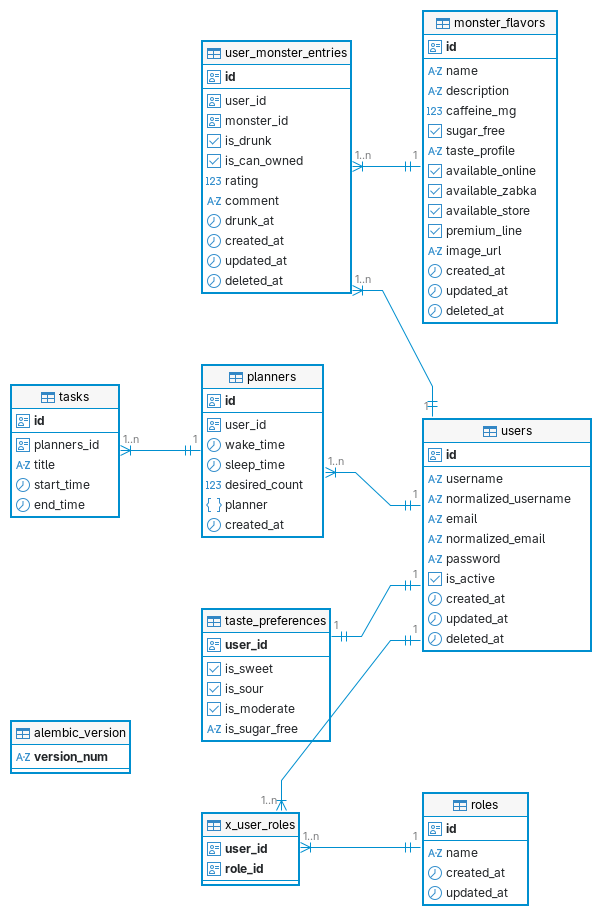
\includegraphics[scale=0.5]{erd.png}
    \caption{Diagram związków encji (ERD) przedstawiający strukturę bazy danych systemu.}
    \label{fig:erd}
\end{figure}

\subsection{Przepływ danych w systemie (DFD)}
Diagram przepływu danych obrazuje interakcje między użytkownikiem a poszczególnymi modułami sztucznej inteligencji oraz proces zapisu danych w persystentnej pamięci masowej (PostgreSQL i S3).

\begin{figure}[H]
    \centering
    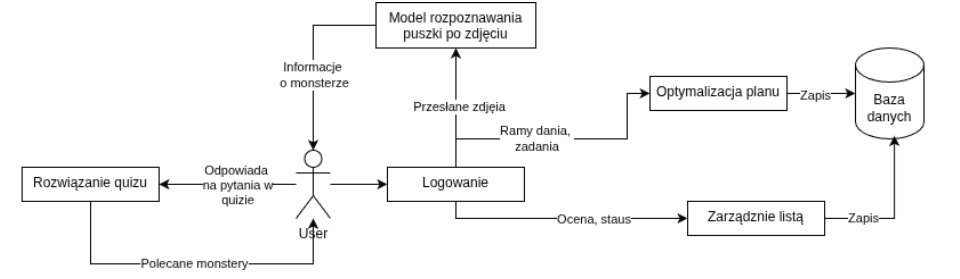
\includegraphics[width=0.9\textwidth]{dfd.png}
    \caption{Diagram przepływu danych (DFD)}
    \label{fig:dfd}
\end{figure}

\section{Instrukcja uruchomienia systemu}
W celu weryfikacji funkcjonalności, system został przystosowany do uruchomienia w środowisku lokalnym przy wykorzystaniu technologii konteneryzacji.

\subsection{Wymagania systemowe}
Przed przystąpieniem do procedury uruchomienia, należy upewnić się, że w systemie zainstalowane są następujące narzędzia:
\begin{itemize}
    \item \textbf{Docker Desktop} (wraz z wtyczką Docker Compose) – do orkiestracji usług backendowych.
    \item \textbf{Node.js} (wersja stabilna) oraz menedżer pakietów \textbf{npm} – do obsługi warstwy frontendowej.
    \item Narzędzie \textbf{git} – do klonowania repozytoriów.
\end{itemize}

\newpage

\subsection{Procedura uruchomienia warstwy Backend}
Moduł serwerowy składa się z kilku powiązanych usług (API, PostgreSQL, MinIO, Mailpit). Proces ich inicjalizacji przebiega następująco:
\begin{enumerate}
    \item Pobranie najnowszej wersji kodu źródłowego z oficjalnego repozytorium: \\ \texttt{https://github.com/Monster-IA-Team/Monster-IA-Backend}
    \item Przejście do katalogu głównego projektu.
    \item Konfiguracja środowiska: Należy utworzyć plik \texttt{.env} na podstawie dostarczonego wzorca \texttt{.env.example}. W sekcji \texttt{API\_JWT\_SECRET\_KEY} należy umieścić wygenerowany klucz bezpieczeństwa dla standardu JWT.
    \item Uruchomienie kontenerów poleceniem: \\ \texttt{docker compose up --build}.
    \item Proces budowania i konfiguracji bazy (w tym migracje \texttt{alembic}) potrwa od 2 do 5 minut. Po tym czasie usługi będą dostępne.
\end{enumerate}

\subsection{Procedura uruchomienia warstwy Frontend}
Aplikacja kliencka (React) uruchamiana jest niezależnie od kontenerów backendowych:
\begin{enumerate}
    \item Pobranie kodu źródłowego frontendu: \\ \texttt{https://github.com/Monster-IA-Team/Monster-IA-Frontend}
    \item Przejście do katalogu projektu w terminalu.
    \item Instalacja niezbędnych zależności projektowych poleceniem: \\ \texttt{npm install}
    \item Uruchomienie serwera deweloperskiego: \\ \texttt{npm run dev}
\end{enumerate}

Po wykonaniu powyższych kroków, aplikacja webowa będzie dostępna pod adresem \texttt{http://localhost:5173}, natomiast dokumentacja interaktywna API (Swagger) pod adresem \texttt{http://localhost:8000/docs}. Szczegółowe informacje techniczne dotyczące konfiguracji poszczególnych modułów znajdują się w plikach \texttt{README.md} w odpowiednich repozytoriach.

\section{Implementacja}

\subsection{Główny framework aplikacyjny (Python i FastAPI)}
Jako fundament warstwy serwerowej wybrano język Python wraz z nowoczesnym frameworkiem FastAPI.
\begin{itemize}
    \item \textbf{Uzasadnienie wyboru:} Python stanowi natywne środowisko dla wiodących bibliotek sztucznej inteligencji (takich jak PyTorch), co eliminuje konieczność tworzenia złożonej architektury mikroserwisowej. FastAPI wybrano ze względu na pełne wsparcie dla operacji asynchronicznych (kluczowe przy przetwarzaniu obrazów) oraz automatyczną walidację danych wejściowych opartą na standardzie Pydantic.
\end{itemize}

\subsection{Wizja Komputerowa i Sieci Neuronowe (PyTorch i TorchVision)}
Moduł rozpoznawania produktów (AI Vision) zrealizowano w oparciu o bibliotekę PyTorch. System wykorzystuje model binarny do detekcji puszki oraz klasyfikator wieloklasowy do rozpoznawania wariantu smakowego.

\begin{itemize}
    \item \textbf{Transfer Learning:} Zamiast trenowania sieci od podstaw, zastosowano uczenie transferowe na architekturach ResNet18 oraz MobileNetV2. Wykorzystanie wag pre-trenowanych na zbiorze ImageNet pozwoliło uzyskać wysoką precyzję przy relatywnie małym zbiorze danych własnych. W procesie uczenia (optymalizator Adam, CrossEntropyLoss) zmodyfikowano jedynie końcową warstwę w pełni połączoną (\texttt{nn.Linear}), dostosowując ją do liczby smaków w systemie.
\end{itemize}

\begin{figure}[H]
    \centering
    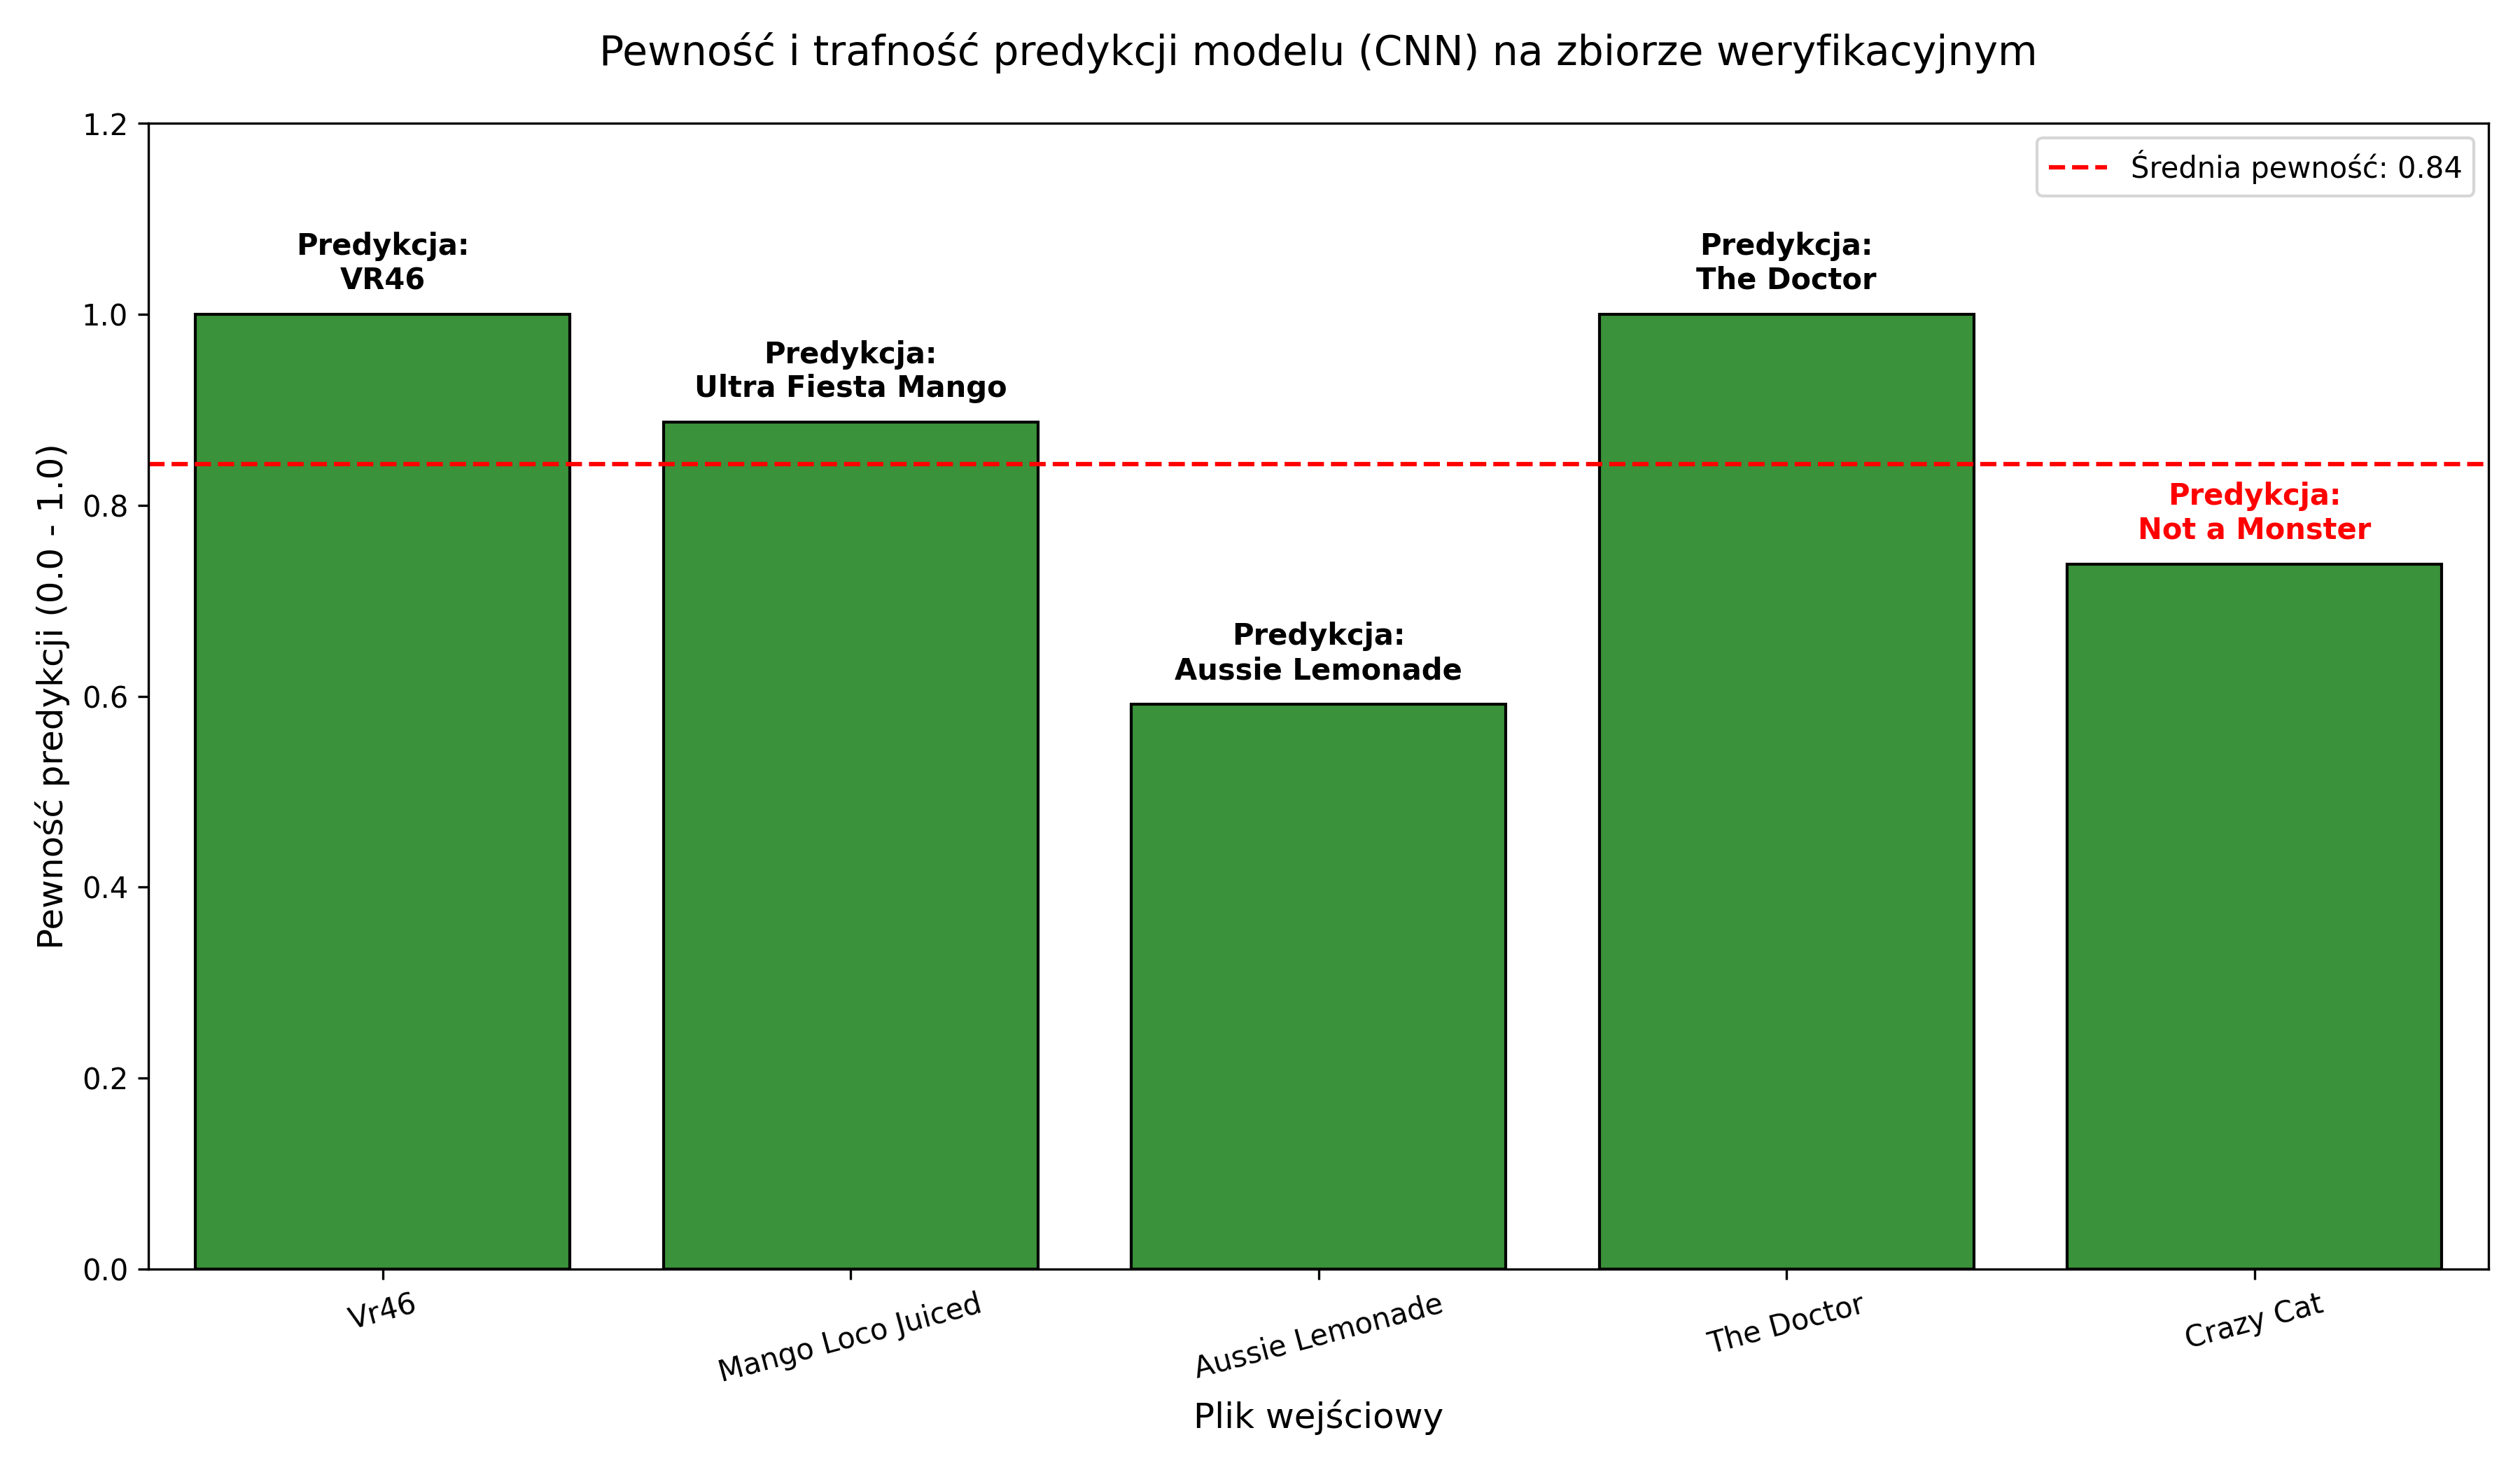
\includegraphics[width=0.85\textwidth]{real_neural_network_confidence.png}
    \caption{Pewność i trafność predykcji modelu wizyjnego na zbiorze weryfikacyjnym.}
    \label{fig:cnn_conf}
\end{figure}

\newpage

\subsection{Optymalizacja Harmonogramów (Natywny Algorytm Genetyczny)}
Silnik wyliczający optymalne godziny spożycia kofeiny opiera się na autorskiej implementacji Algorytmu Genetycznego w języku Python.

\begin{itemize}
    \item \textbf{Logika ewolucyjna:} Zastosowano selekcję turniejową oraz mutację opartą o rozkład Gaussa, co pozwala na precyzyjne przeszukiwanie przestrzeni rozwiązań bez utraty stabilności. Funkcja Fitness uwzględnia kary za nakładanie się dawek (overlap penalty) oraz nagradza rozwiązania maksymalizujące wydajność w oknach czasowych zdefiniowanych zadań.
\end{itemize}

\begin{figure}[H]
    \centering
    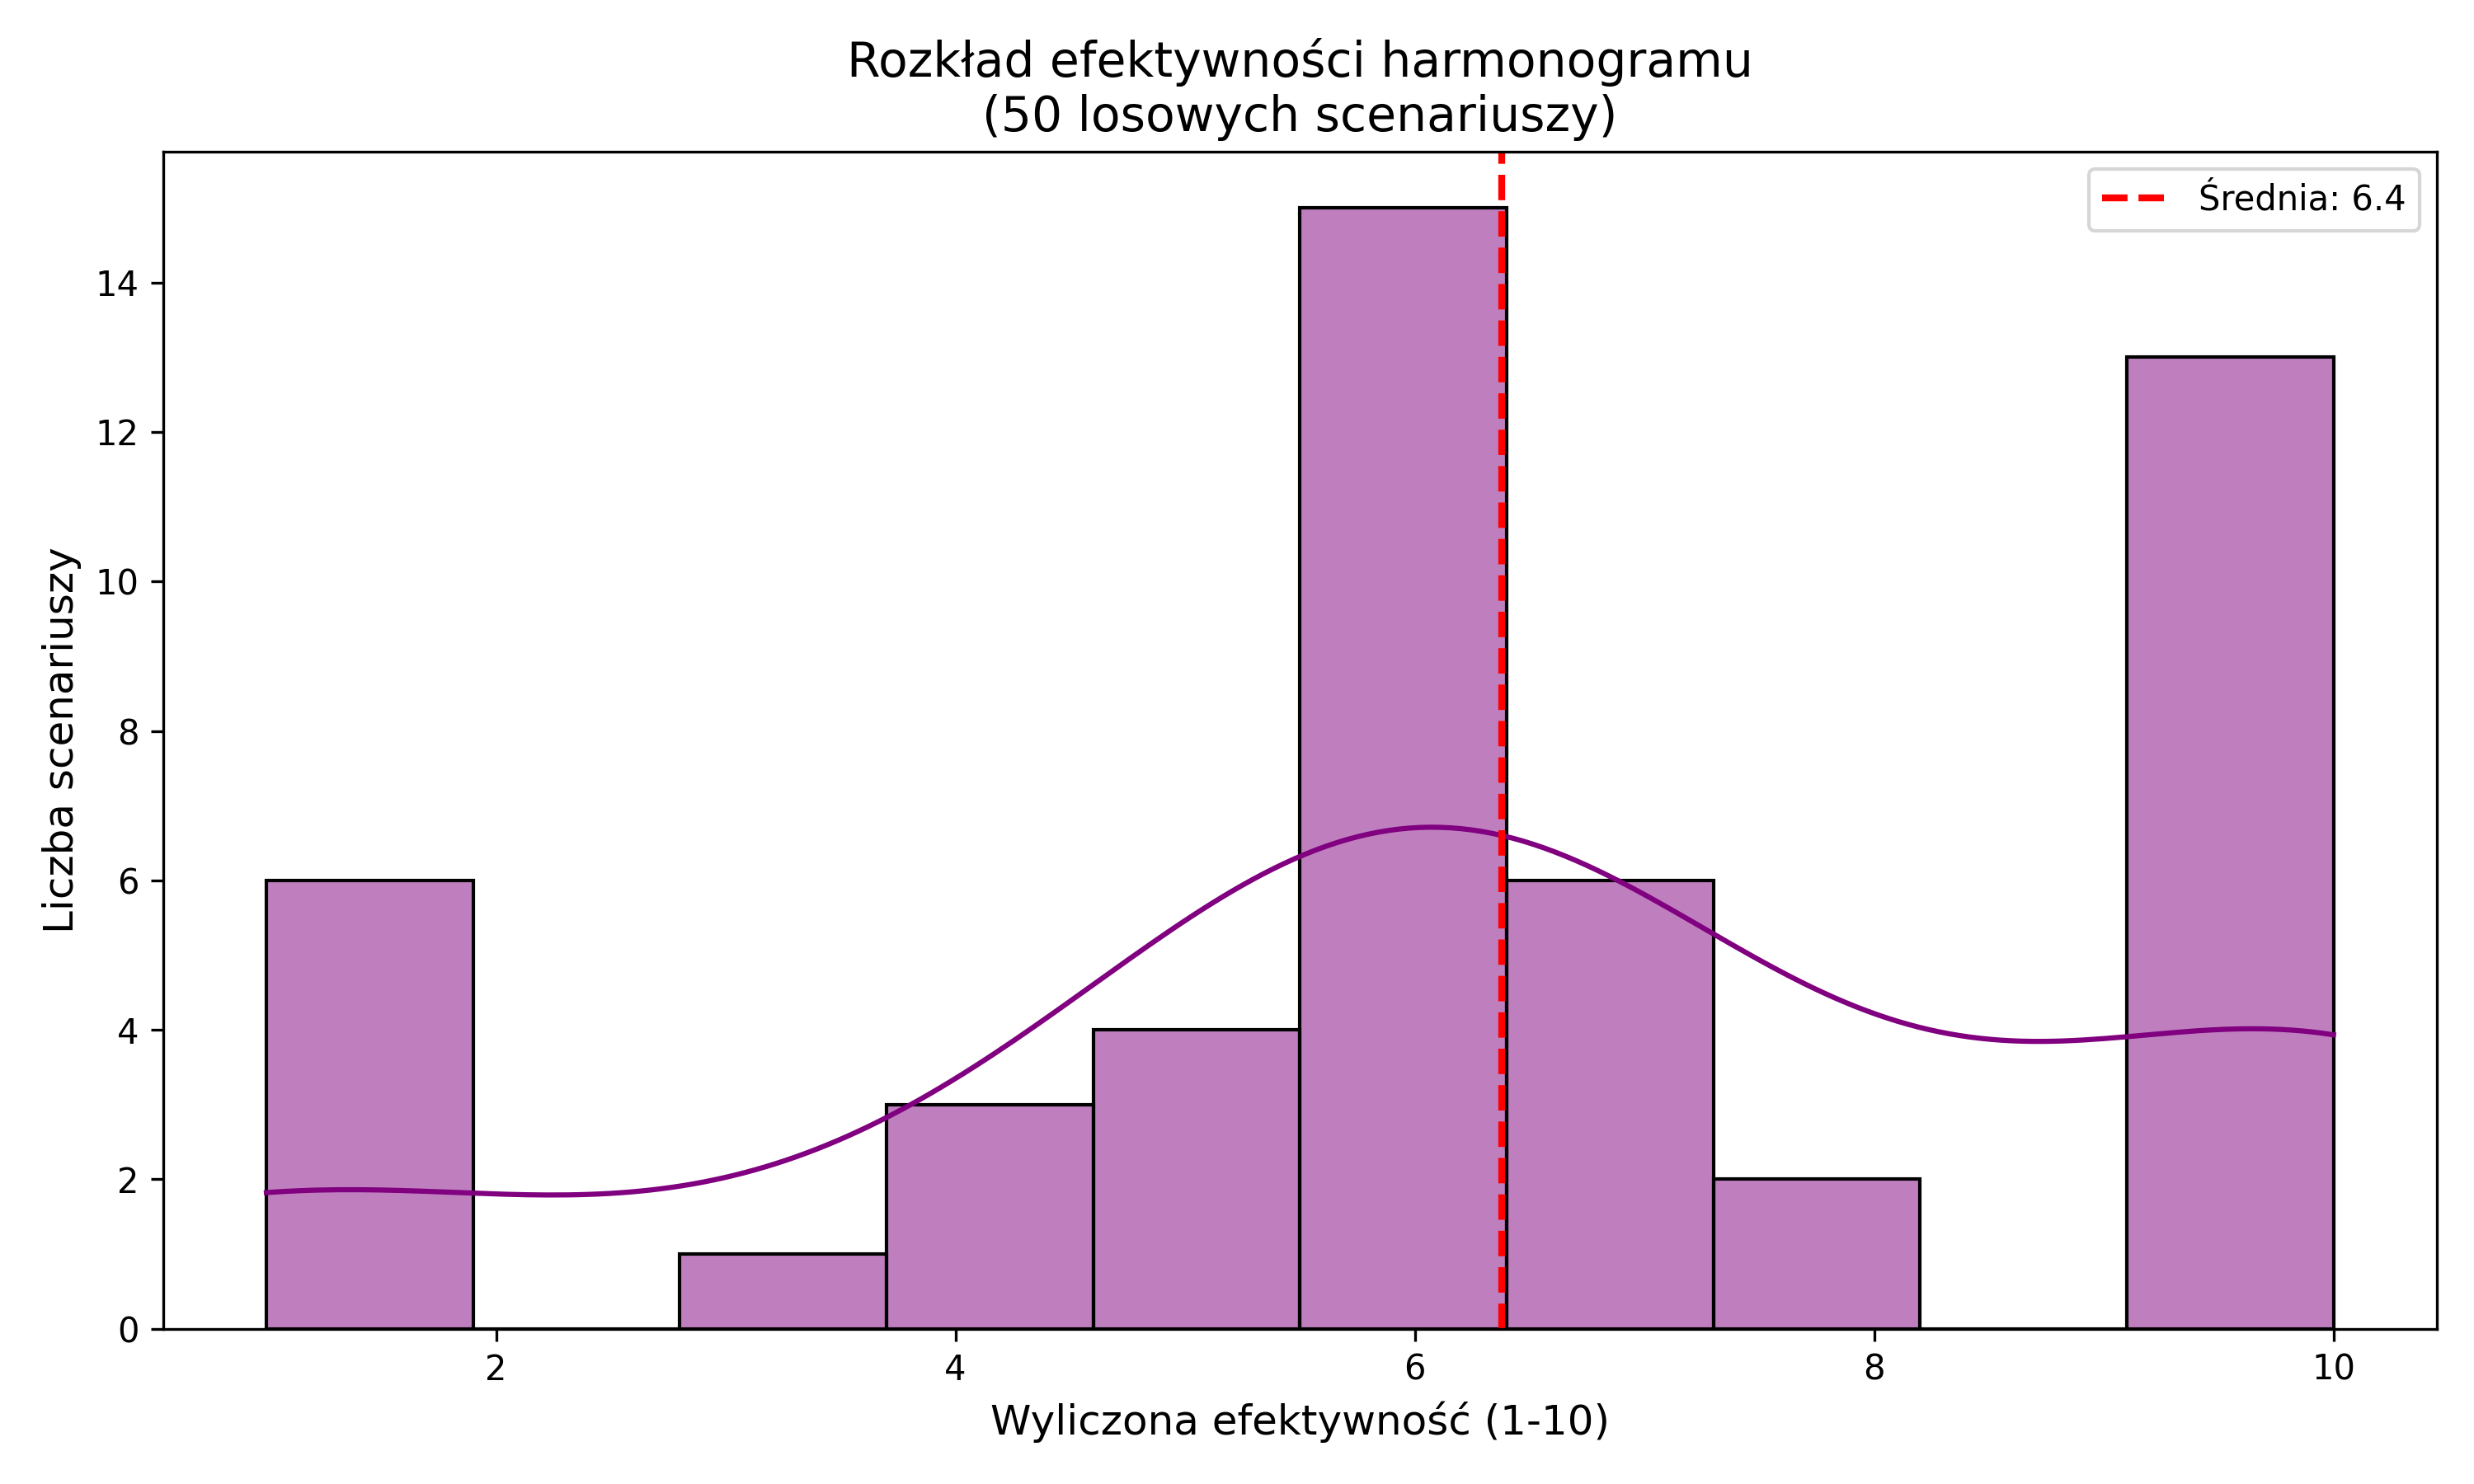
\includegraphics[width=0.75\textwidth]{real_genetic_robustness_hist.png}
    \caption{Histogram rozkładu funkcji Fitness wykazujący wysoką zbieżność algorytmu genetycznego.}
    \label{fig:ga_hist}
\end{figure}

\begin{figure}[H]
    \centering
    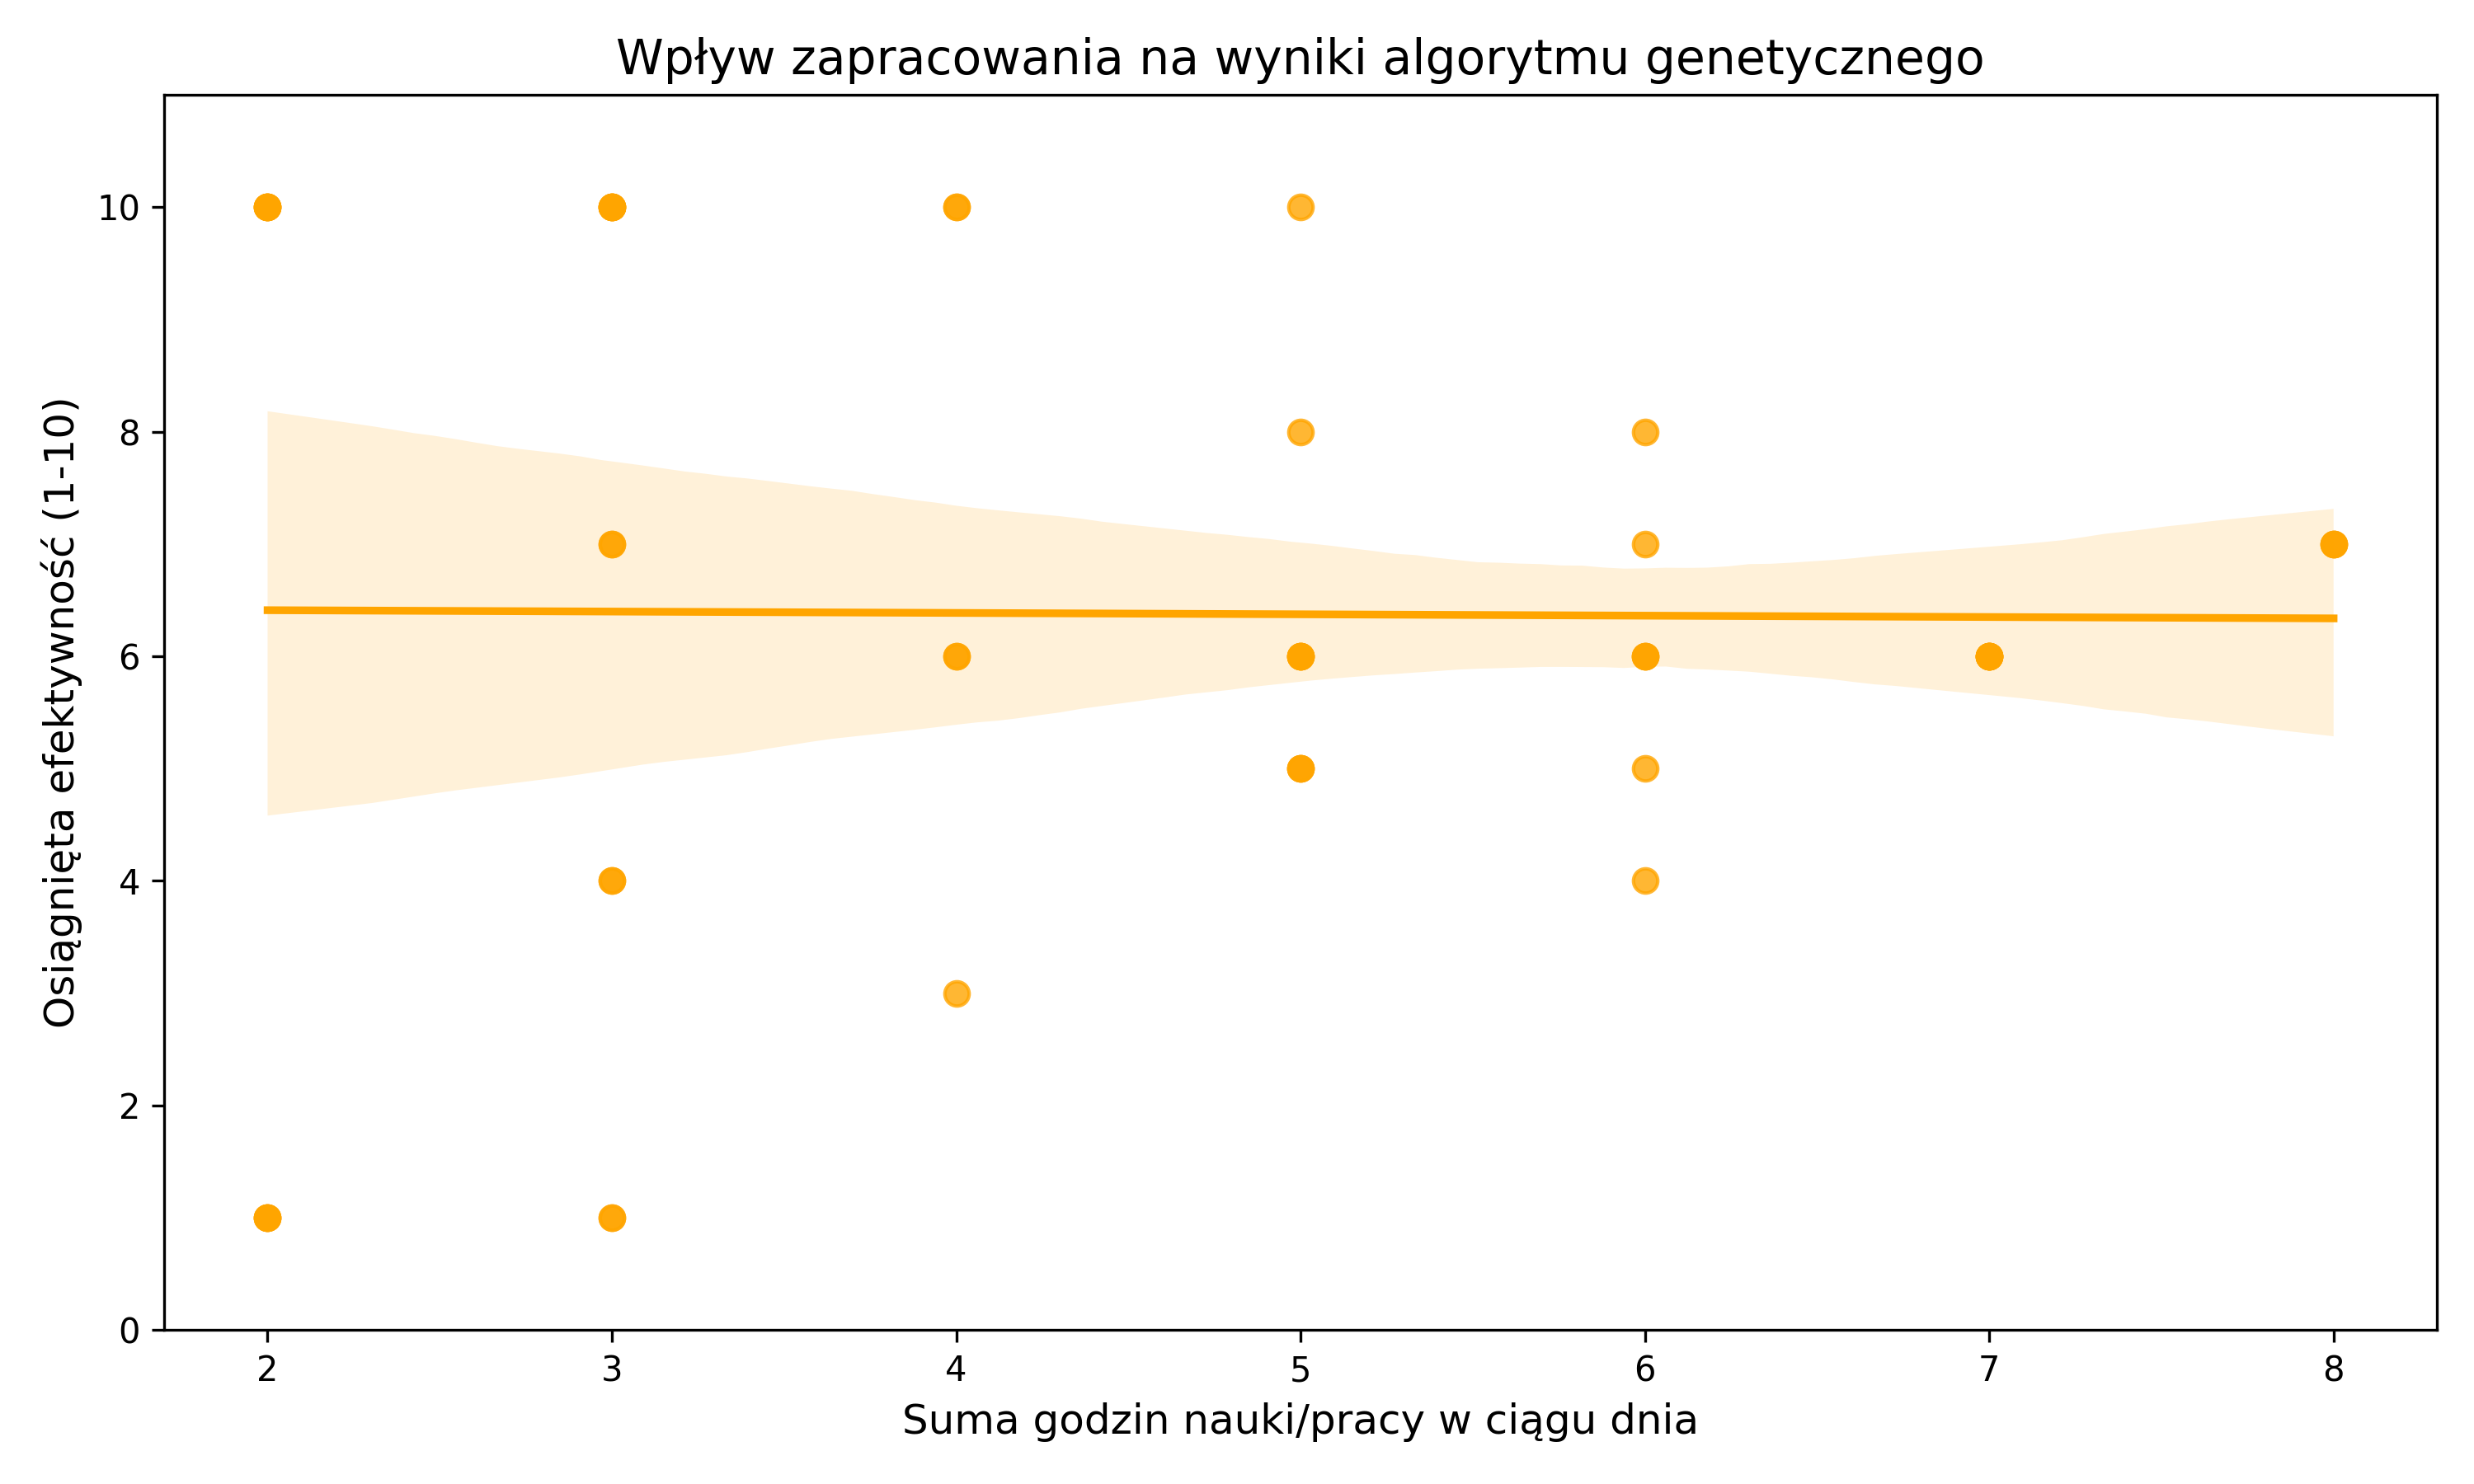
\includegraphics[width=0.75\textwidth]{real_genetic_robustness_scatter.png}
    \caption{Diagram wpływu zapracowania (liczby zadań) na efektywność wygenerowanego planu.}
    \label{fig:ga_scatter}
\end{figure}

\newpage

\subsection{System Rekomendacyjny (Drzewo Decyzyjne)}
Moduł quizu opiera się na deterministycznym drzewie decyzyjnym zdefiniowanym w formacie JSON. 

\begin{itemize}
    \item \textbf{Przetwarzanie regułowe:} Zastosowanie operacji na zbiorach (intersection) pozwala na błyskawiczne filtrowanie bazy produktów (smaków) w oparciu o kryteria takie jak typ sklepu, budżet czy profil smakowy. Oddzielenie logiki drzewa od kodu pozwala na modyfikację reguł bez ingerencji w strukturę aplikacji.
\end{itemize}

\begin{figure}[H]
    \centering
    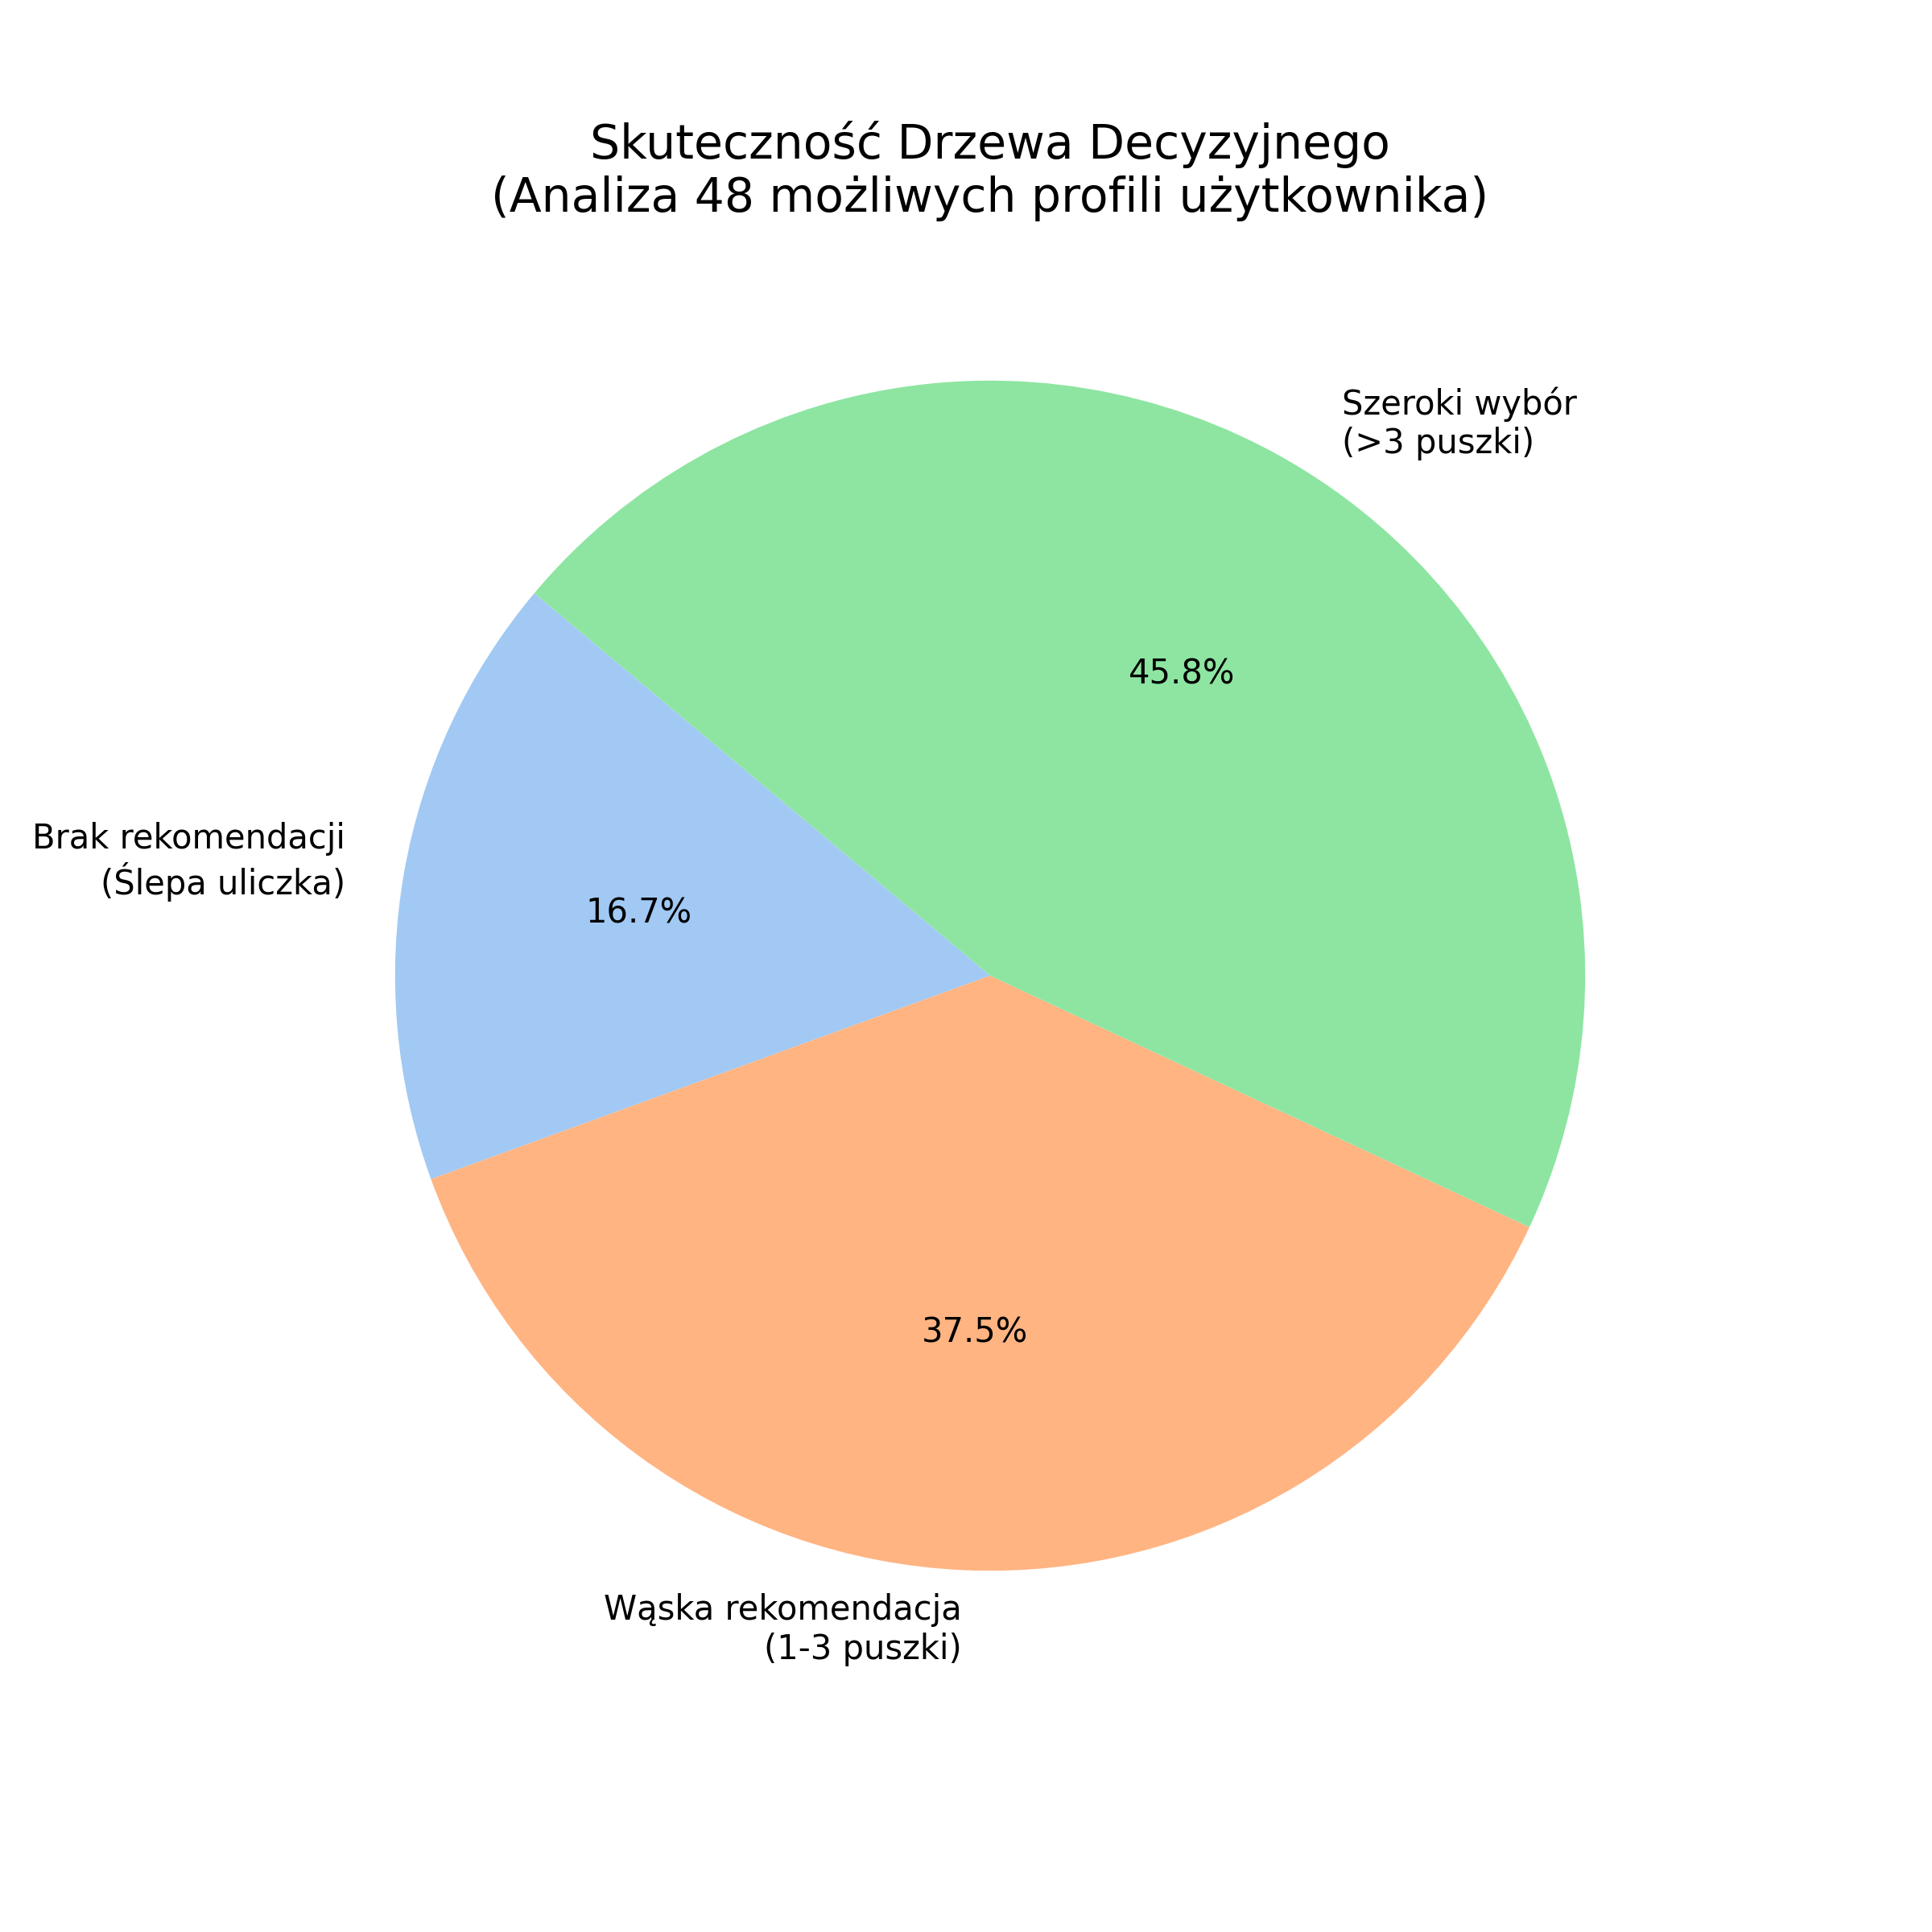
\includegraphics[width=0.75\textwidth]{real_expert_system_coverage.png}
    \caption{Analiza pokrycia systemu eksperckiego: liczba rekomendacji dla różnych profili użytkowników.}
    \label{fig:expert_cov}
\end{figure}

\begin{figure}[H]
    \centering
    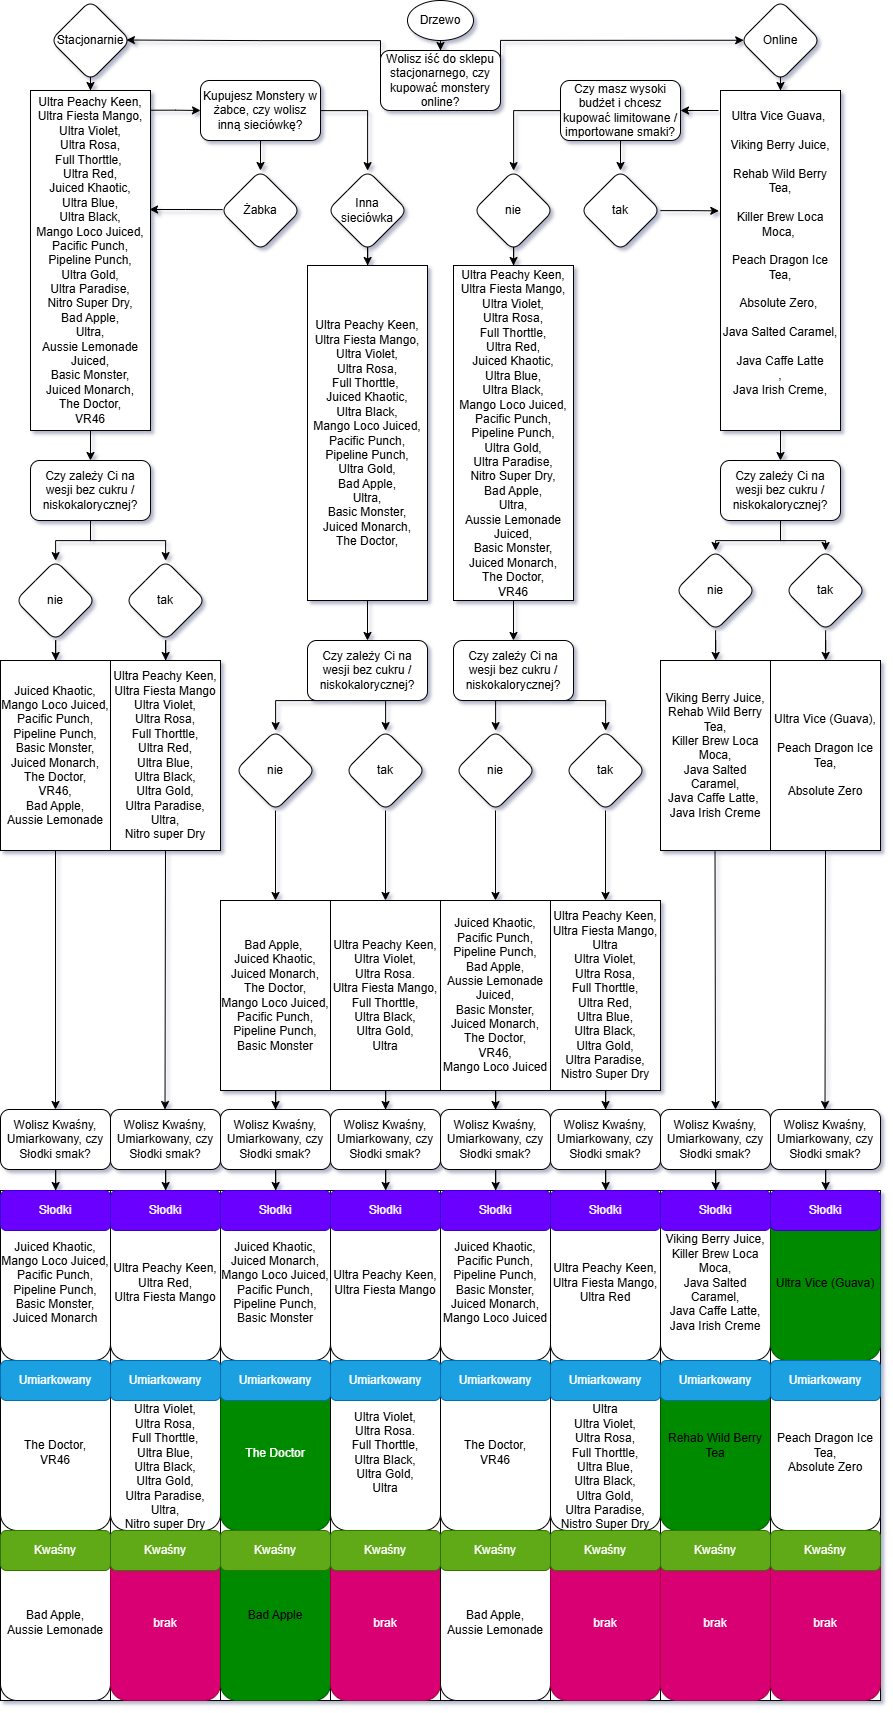
\includegraphics[width=15cm,height=23cm]{decision_tree.png}
    \caption{Graficzna reprezentacja drzewa decyzyjnego wykorzystywanego w module rekomendacji.}
    \label{fig:tree_graf}
\end{figure} 

\section{Kluczowe fragmenty kodu źródłowego}
W celu zaprezentowania technicznej implementacji opisanych wcześniej modeli, poniżej zamieszczono kluczowe fragmenty logiki biznesowej.

\subsection{Implementacja Uczenia Transferowego (Transfer Learning)}
Poniższy fragment kodu z modułu uczącego udowadnia zastosowanie techniki Transfer Learningu. Oryginalne wagi modelu pre-trenowanego na zbiorze ImageNet (np. ResNet18) zostają zamrożone, a optymalizacji podlega jedynie nowo zainicjowana warstwa w pełni połączona (\texttt{nn.Linear}), dostosowana do liczby klas decyzyjnych w systemie.

\begin{lstlisting}[language=Python, caption=Funkcja inicjująca architekturę modelu (plik train\_binary.py), label=lst:transfer_learning]
def get_model(name, n_classes, pretrained=True):
    if name == "resnet18":
        model = models.resnet18(weights='DEFAULT' if pretrained else None)
        for param in model.parameters():
            param.requires_grad = False

        num_ftrs = model.fc.in_features
        model.fc = nn.Linear(num_ftrs, n_classes)
        
    elif name == "mobilenet_v2":
        model = models.mobilenet_v2(weights='DEFAULT' if pretrained else None)
        for param in model.parameters():
            param.requires_grad = False
        num_ftrs = model.classifier[1].in_features
        model.classifier[1] = nn.Linear(num_ftrs, n_classes)
    else:
        raise ValueError("Unknown model: " + name)
    return model
\end{lstlisting}

\newpage

\subsection{Dwuetapowa inferencja modelu wizyjnego w API}
Przetwarzanie zapytań od użytkownika oparto na dwuetapowym procesie wnioskowania. Wykorzystanie bloku \texttt{torch.no\_grad()} optymalizuje pamięć serwera poprzez wyłączenie śledzenia gradientów. Model binarny pełni rolę filtra brzegowego, zabezpieczając system przed błędnymi danymi wejściowymi.

\begin{lstlisting}[language=Python, caption=Logika predykcji w serwisie backendowym (plik prediction\_services.py), label=lst:inference]
def predict(self, img_bytes: bytes) -> PredictionResponse:
    # ... (Transformacja zdjecia do tensora img_t) ...
    
            with torch.no_grad():
            bin_out = self.binary_model(img_t)
            if bin_out.dim() == 1:
                bin_out = bin_out.unsqueeze(0)
                
            bin_probs = torch.nn.functional.softmax(bin_out, dim=1).squeeze()
            bin_conf_val, bin_idx_val = torch.max(bin_probs, dim=0)
            best_binary_label = self.binary_classes[bin_idx_val.item()]

            if best_binary_label == "Not_Monster":
                return PredictionResponse(
                    label="This image does not contain a monster.",
                    confidence=float(bin_conf_val.item()),
                    prediction=[],
                    num_classes=len(self.binary_classes)
                )

            out = self.model(img_t)
            
            if out.dim() == 1:
                out = out.unsqueeze(0)
                
            probs = torch.nn.functional.softmax(out, dim=1).squeeze()
            conf_val, idx_val = torch.max(probs, dim=0)
            best_label = self.classes[idx_val.item()]
            best_conf = float(conf_val.item())
        
        # ... (Formatowanie i sortowanie wynikow) ...
\end{lstlisting}

\newpage

\subsection{Funkcja oceny (Fitness) w Algorytmie Genetycznym}
Kluczowym elementem optymalizacji harmonogramu jest odpowiednio zaprojektowana funkcja przystosowania. Zaprezentowana poniżej metoda ocenia każdego osobnika (potencjalny plan spożycia), przyznając punkty za pokrycie zaplanowanych zadań (pracy/nauki) oknem działania stymulanta, a jednocześnie nakładając surowe kary matematyczne za zjawisko zbyt częstego spożycia (nakładanie się na siebie dawek).

\begin{lstlisting}[language=Python, caption=Implementacja funkcji fitness dla harmonogramu (plik schedule\_services.py), label=lst:ga_fitness]
    def _calculate_fitness(self, individual: List[Tuple[float, float]],
                           wake_float: float, sleep_float: float,
                           task_intervals: List[Tuple[float, float]]) -> float:
        if not self._is_valid_individual(individual, wake_float, sleep_float):
            return INVALID_FITNESS

        intervals = [(start, start + effect) for start, effect in individual]
        penalty = sum(
            IntervalUtils.overlap_length(interval_a[0], interval_a[1], interval_b[0], interval_b[1]) * self.overlap_penalty
            for idx_a, interval_a in enumerate(intervals)
            for interval_b in intervals[idx_a + 1:]
        )
        merged_intervals = IntervalUtils.merge(intervals)
        covered = sum(
            IntervalUtils.overlap_length(interval_start, interval_end, task_start, task_end)
            for task_start, task_end in task_intervals
            for interval_start, interval_end in merged_intervals
        )
        return covered - penalty
\end{lstlisting}

\subsection{Mutacja z wykorzystaniem rozkładu Gaussa}
W celu uniknięcia utknięcia algorytmu w minimach lokalnych, zastosowano zaawansowany operator mutacji. W przeciwieństwie do czysto losowych modyfikacji, algorytm wykorzystuje rozkład normalny (Gaussa), co pozwala na ewolucyjne, delikatne przesuwanie godzin spożycia. Metoda ta ściśle pilnuje również twardych ograniczeń fizjologicznych – np. bufora czasowego przed snem (\texttt{buffer\_hours}).

\begin{lstlisting}[language=Python, caption=Operator mutacji Gaussa z zachowaniem ograniczen fizjologicznych (plik schedule\_services.py), label=lst:ga_mutate]
    def _mutate(self, individual: List[Tuple[float, float]], wake_float: float,
                sleep_float: float, monster_count: int, mutation_rate: float) -> List[Tuple[float, float]]:
        mutated = []
        for i, (start, effect) in enumerate(individual):
            if random.random() < mutation_rate:
                start += random.gauss(0, self.gaussian_std)
            if random.random() < mutation_rate:
                effect += random.gauss(0, self.gaussian_std)

            start = max(wake_float, min(start, sleep_float - self.max_effect))
            effect = max(self.min_effect, min(effect, self.max_effect))

            if i > 0:
                start = max(start, mutated[-1][0] + self.min_gap)
            if start + effect > sleep_float - self.buffer_hours:
                effect = max(self.min_effect, sleep_float - self.buffer_hours - start)

            mutated.append((start, effect))
        return mutated
\end{lstlisting}

\subsection{Silnik wnioskujący Systemu Eksperckiego}
Moduł rekomendacyjny zaimplementowano jako klasyczny system ekspercki oparty na drzewie decyzyjnym. Baza wiedzy (reguły i pytania) została odseparowana od logiki biznesowej i jest przechowywana w strukturze JSON. 

Poniższy fragment pliku \texttt{tree.json} obrazuje strukturę pojedynczego węzła decyzyjnego. Każda odpowiedź zawiera tablicę \texttt{filter}, która określa pulę napojów spełniających dane kryterium, oraz zagnieżdżone kolejne pytanie do użytkownika.

\begin{lstlisting}[language=json, caption=Fragment bazy wiedzy reprezentującej drzewo decyzyjne (plik tree.json), label=lst:tree_json]
{
  "question": "Wolisz iść do sklepu stacjonarnego, czy zamawiać Monster online?",
  "answers": {
    "Stacjonarnie": {
      "filter": [
        "Ultra Peachy Keen",
        "Ultra Fiesta Mango",
        "Juiced Khaotic",
        "Pipeline Punch"
      ],
      "question": "Kupujesz Monstery w Żabce, czy wolisz inną sieciówkę?",
      "answers": { ... }
    }
  }
}
\end{lstlisting}

Aby zoptymalizować proces filtrowania bazy napojów (ok. 30 różnych smaków), silnik wnioskujący zaimplementowany w języku Python nie przeszukuje relacyjnej bazy danych przy każdym pytaniu. Zamiast tego, wykorzystuje wysokowydajne operacje matematyczne na zbiorach (\texttt{set.intersection}), co gwarantuje złożoność obliczeniową pozwalającą na natychmiastowe zwrócenie wyniku.

\begin{lstlisting}[language=Python, caption=Logika silnika wnioskującego w Pythonie (plik quiz\_services.py), label=lst:expert_engine]
def get_answers(self, answers: QuizAnswersRequest) -> list[str]:
    candidates = set(self.monster_list)
    
    shop_key = "Stacjonarnie" if answers.shop_type == 0 else "Online"
    node = self.tree.get("answers", {}).get(shop_key, {})
    if "filter" in node:
        candidates = candidates.intersection(set(node["filter"]))
        
    if answers.shop_type == 0:
        sub_key = "Żabka" if answers.is_zabka else "inne"
    else:
        sub_key = "yes" if answers.high_budget else "no"
        
    node = node.get("answers", {}).get(sub_key, {})
    if "filter" in node:
        candidates = candidates.intersection(set(node["filter"]))
        
    # ... (kolejne kroki schodzenia w glab drzewa, np. zawartosc cukru) ...
        
    # Zwrocenie przefiltrowanej, dopasowanej listy napojow
    return list(candidates)
\end{lstlisting}

\section{Prezentacja interfejsu systemu}
Aby udowodnić poprawne zintegrowanie modułów sztucznej inteligencji z warstwą wizualną i serwerową, poniżej zaprezentowano zrzuty ekranu z działającego systemu.

\subsection{Aplikacja Frontend (Widok Użytkownika)}
To są przykładowe widoki z aplikacji
\begin{figure}[H]
    \centering
    
\includegraphics[width=1\textwidth]{start_page.png}
    \caption{Strona główna}
    \label{fig:frontend}
\end{figure}

\begin{figure}[H]
    \centering
    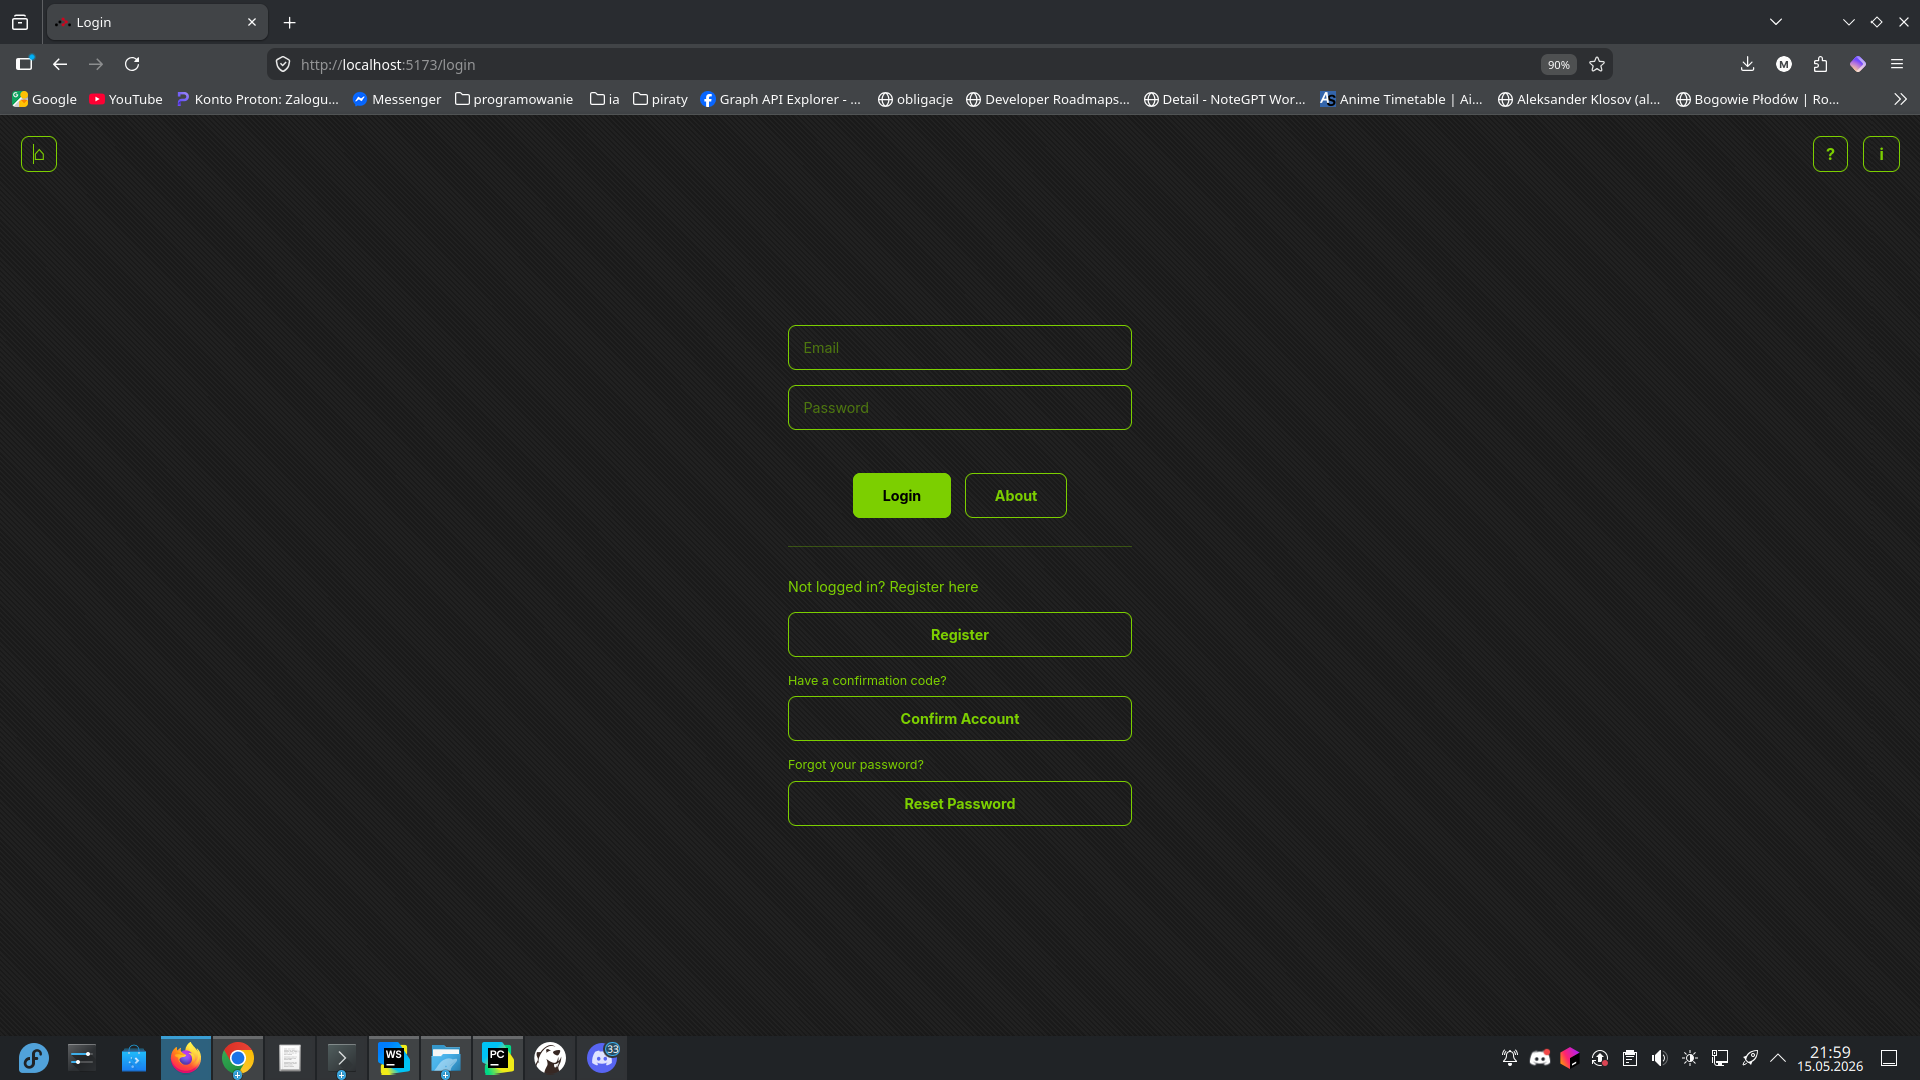
\includegraphics[width=1\textwidth]{login_page.png}
    \caption{Strona logowania}
    \label{fig:frontend}
\end{figure}

\begin{figure}[H]
    \centering
    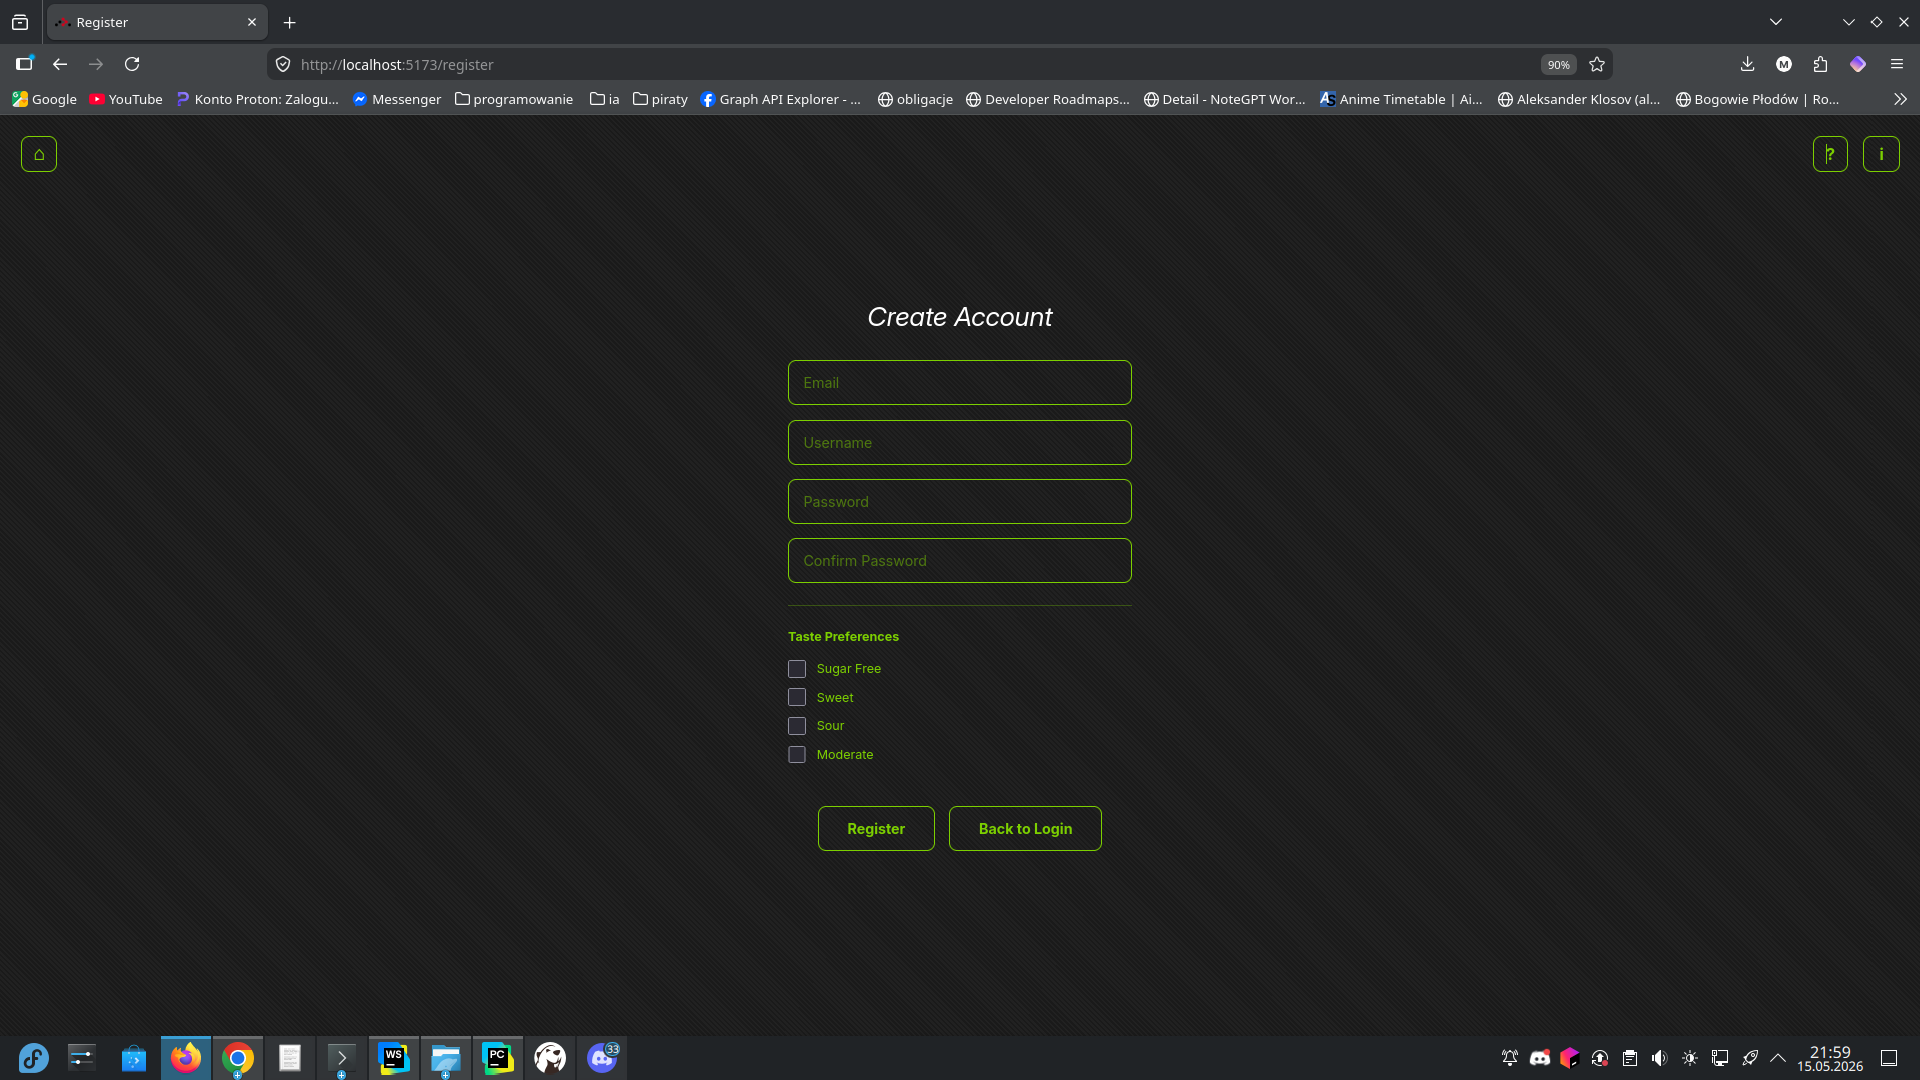
\includegraphics[width=1\textwidth]{register_page.png}
    \caption{Strona rejstracji}
    \label{fig:frontend}
\end{figure}

\begin{figure}[H]
    \centering
    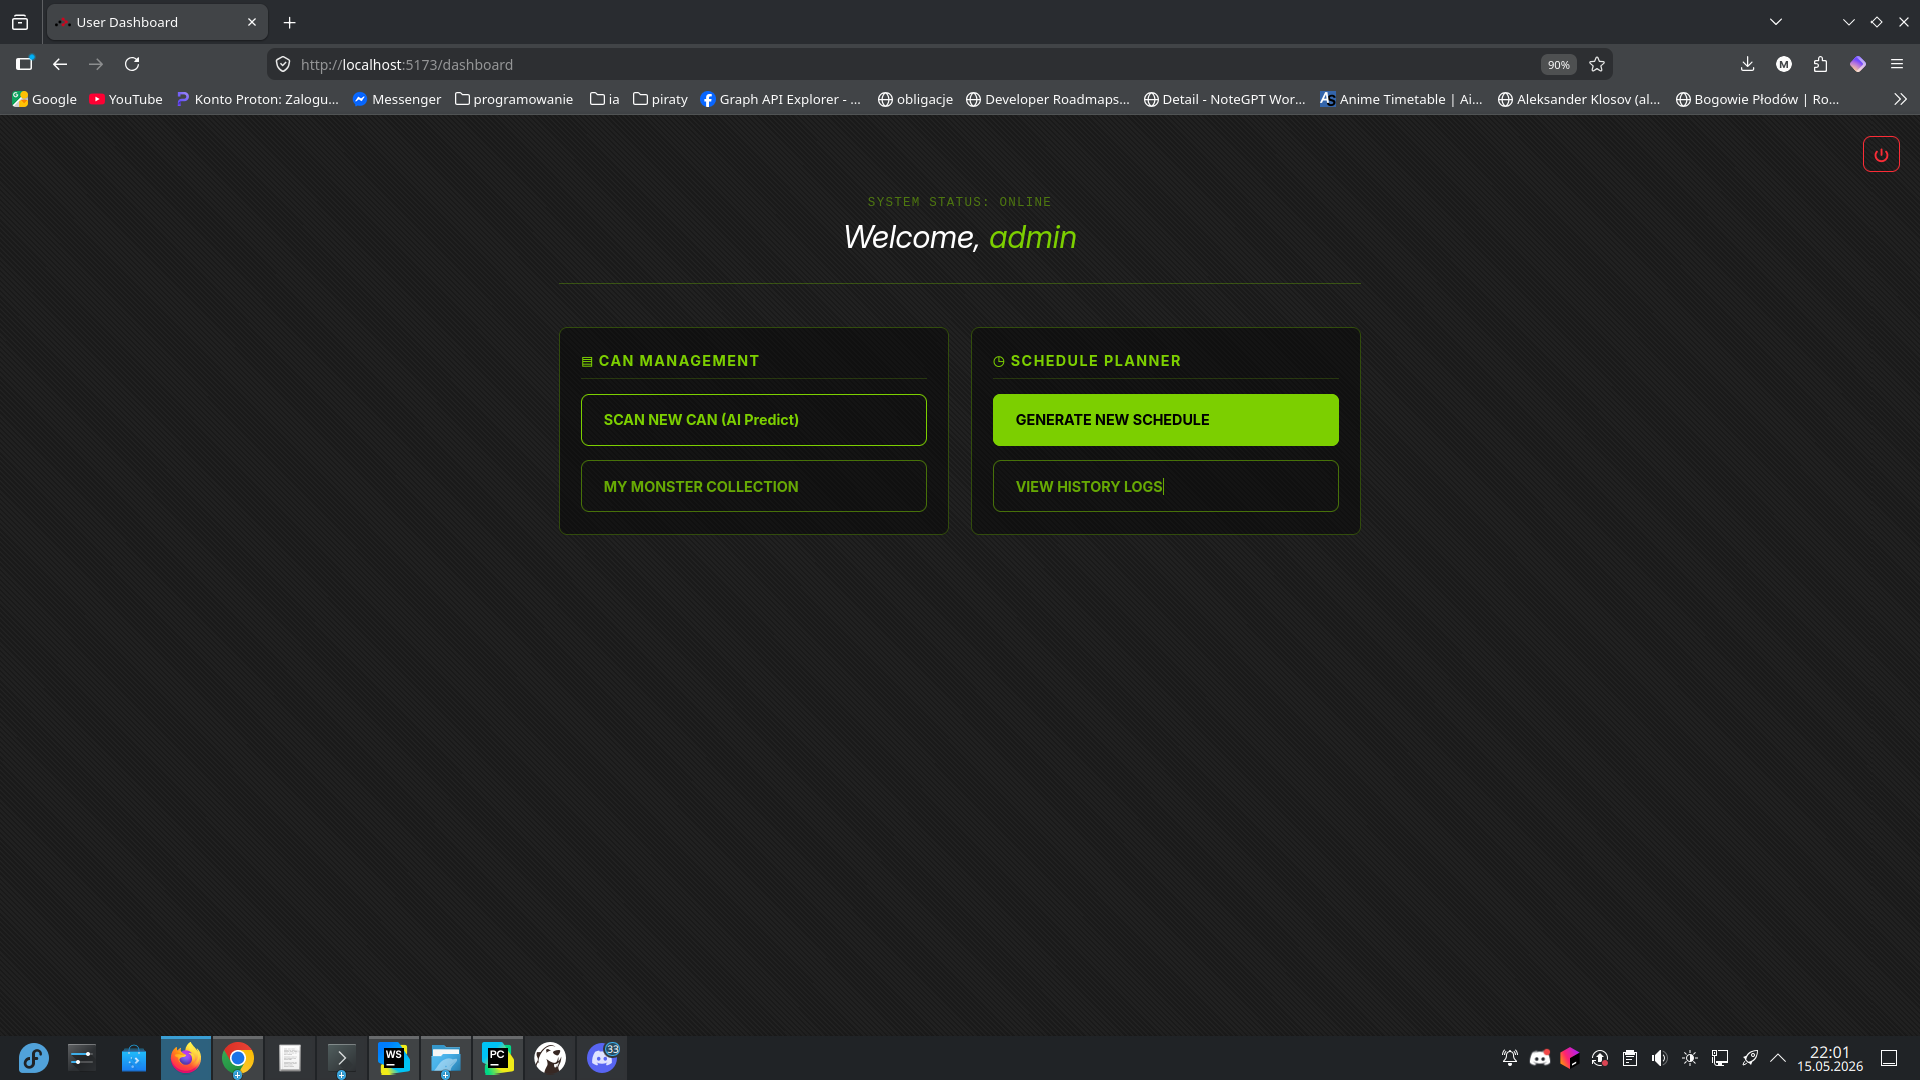
\includegraphics[width=1\textwidth]{user_dashboard.png}
    \caption{Panel użytkownika}
    \label{fig:frontend}
\end{figure}

\begin{figure}[H]
    \centering
    
\includegraphics[width=1\textwidth]{prediction_page.png}
    \caption{Strona do przesyłania zdjęcia puszki do predykcji}
    \label{fig:frontend}
\end{figure}

\begin{figure}[H]
    \centering
    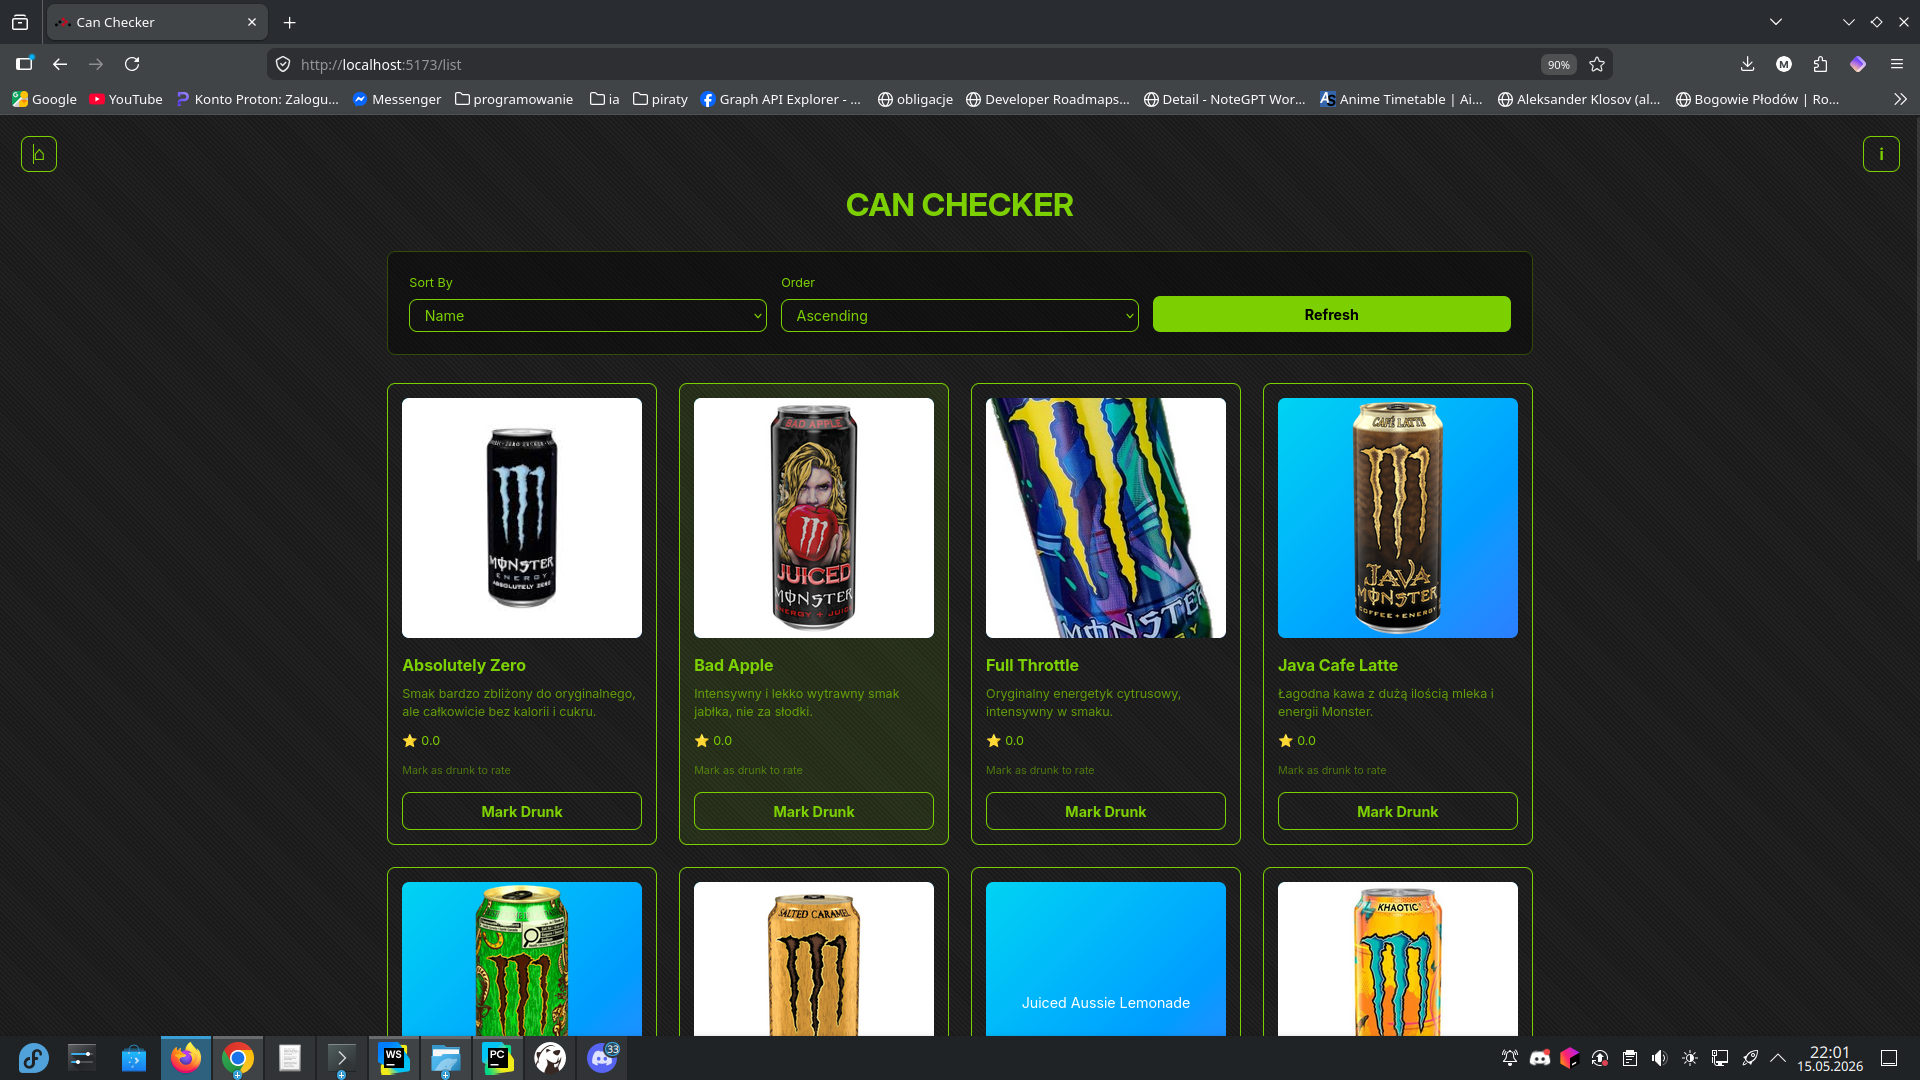
\includegraphics[width=1\textwidth]{monster_list.png}
    \caption{Strona listy monsterów}
    \label{fig:frontend}
\end{figure}

\begin{figure}[H]
    \centering
    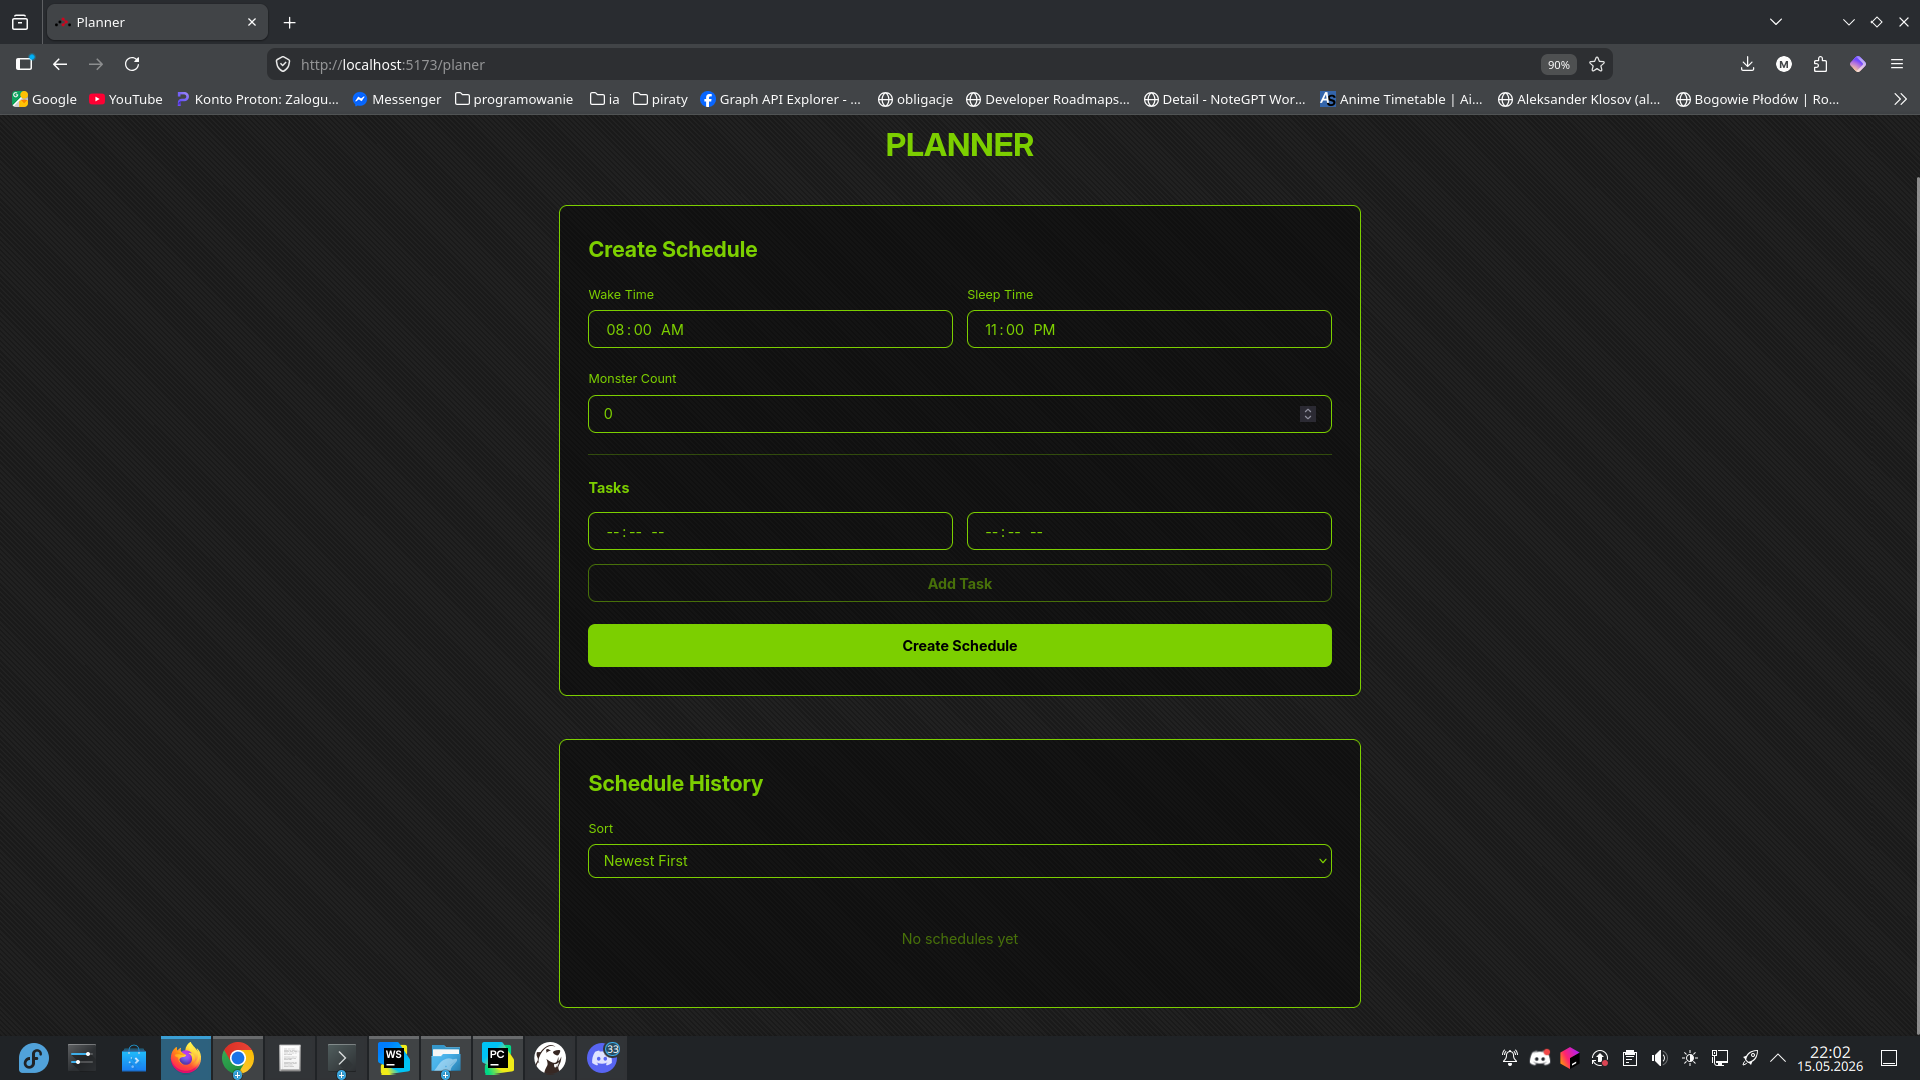
\includegraphics[width=1\textwidth]{planer_generator.png}
    \caption{Strona generatora planera}
    \label{fig:frontend}
\end{figure}

\begin{figure}[H]
    \centering
    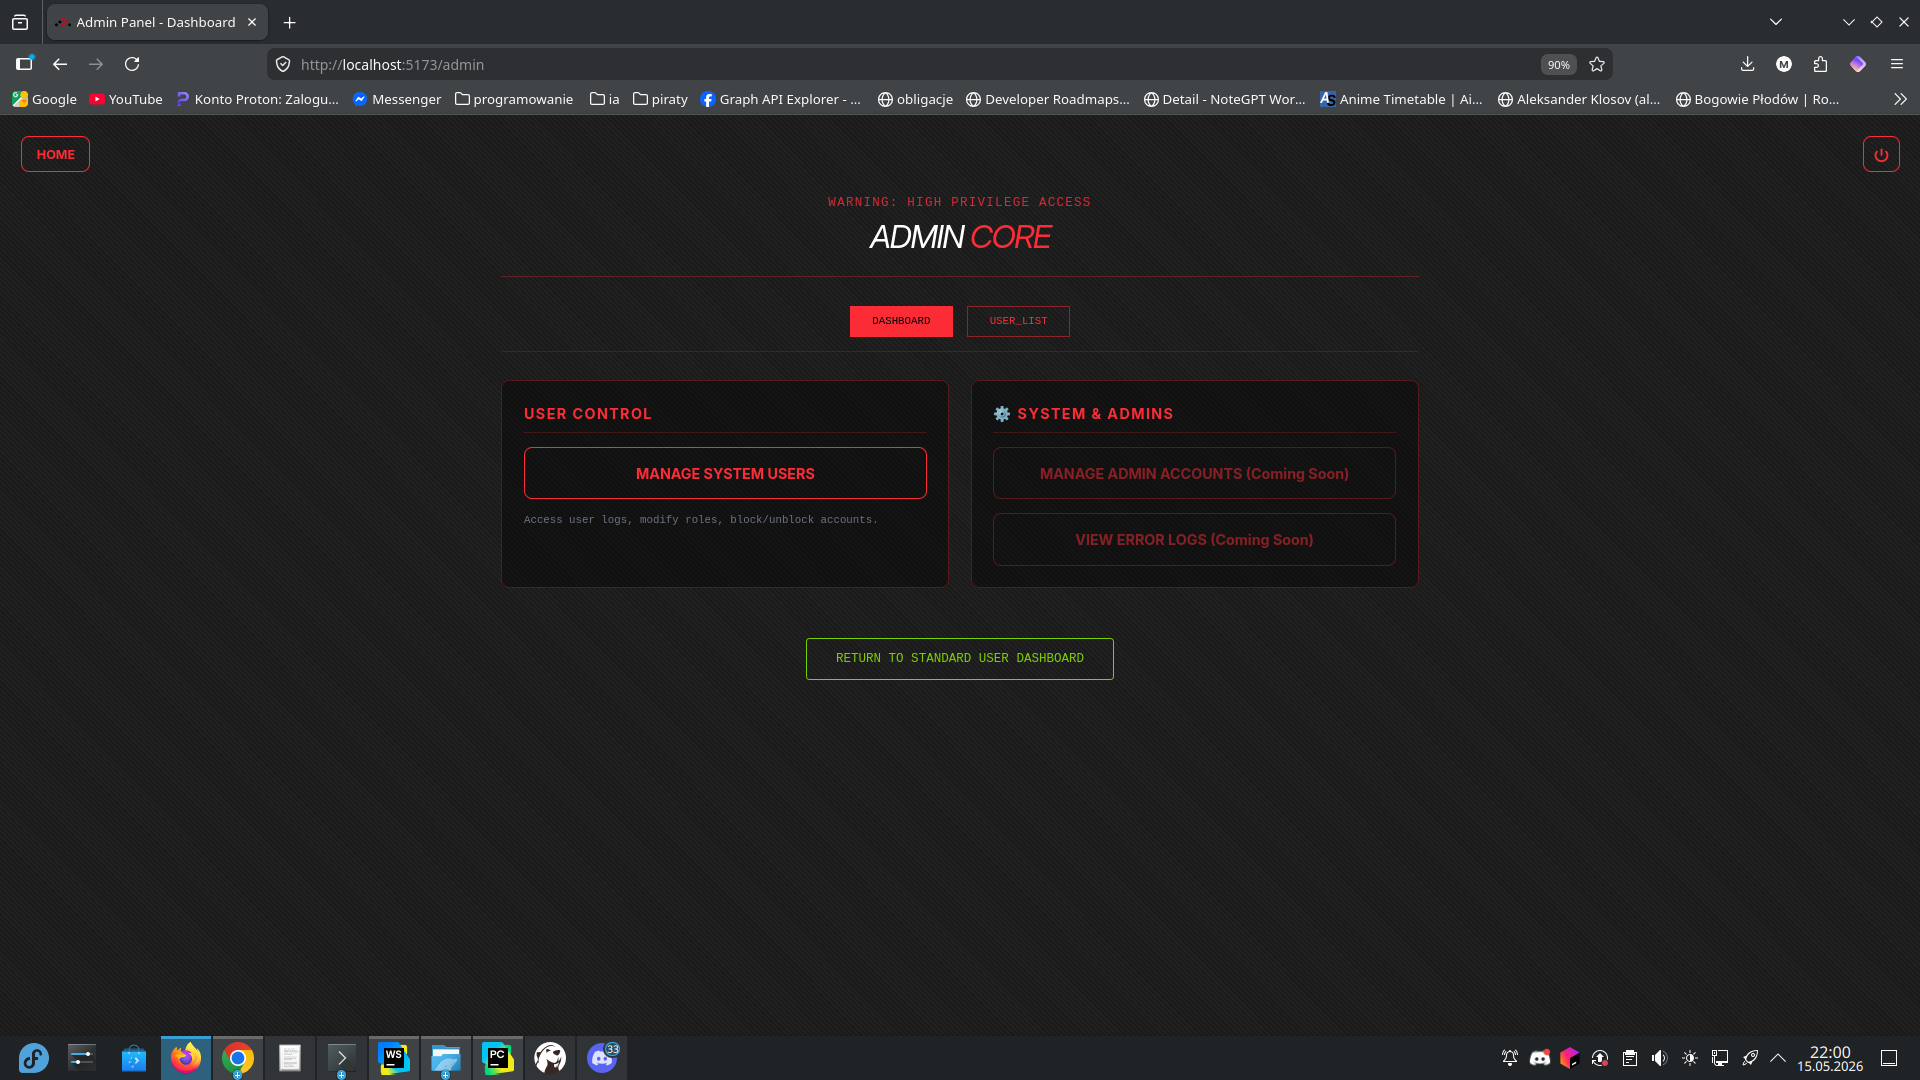
\includegraphics[width=1\textwidth]{admin_dashboard.png}
    \caption{Panel administratora}
    \label{fig:frontend}
\end{figure}

\begin{figure}[H]
    \centering
    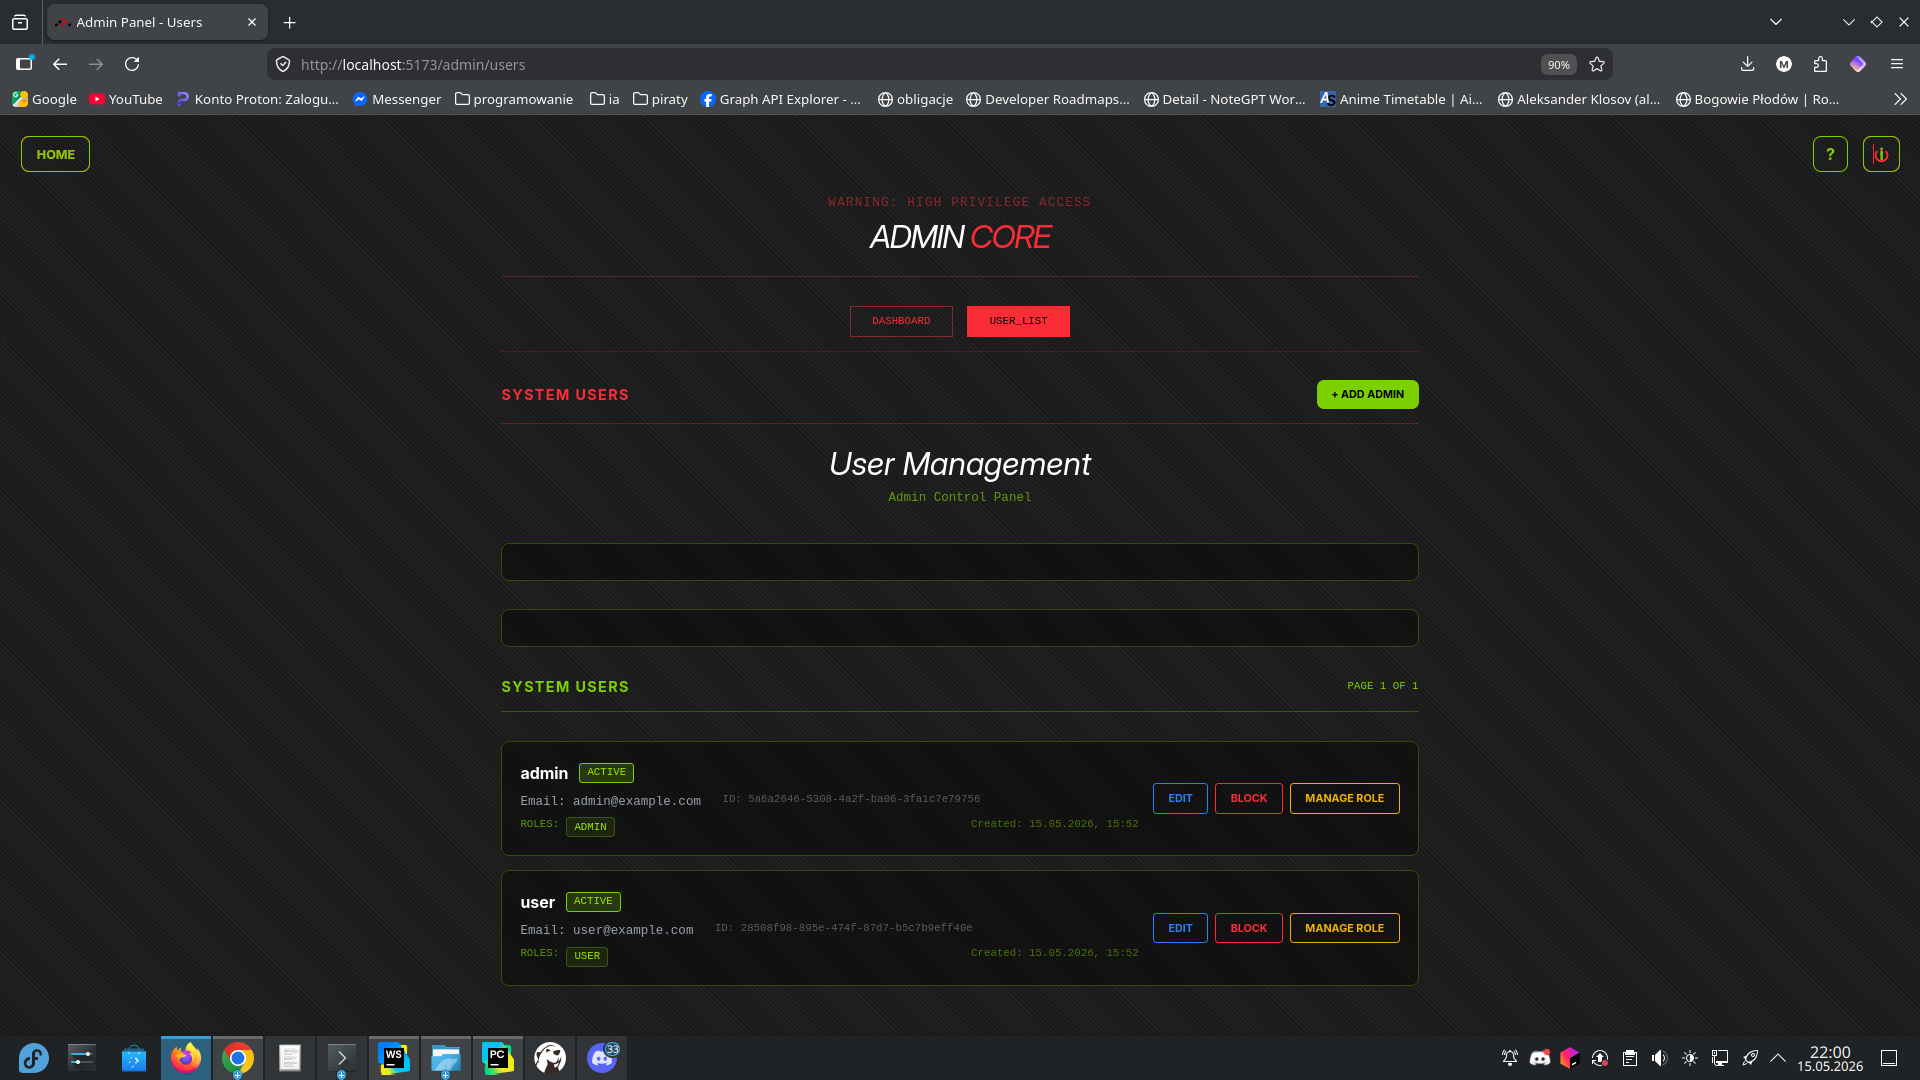
\includegraphics[width=1\textwidth]{user_managment.png}
    \caption{Zarządzanie użytkownikami}
    \label{fig:frontend}
\end{figure}

\subsection{Aplikacja Backend (Dokumentacja API Swagger)}
\begin{figure}[H]
    \centering
    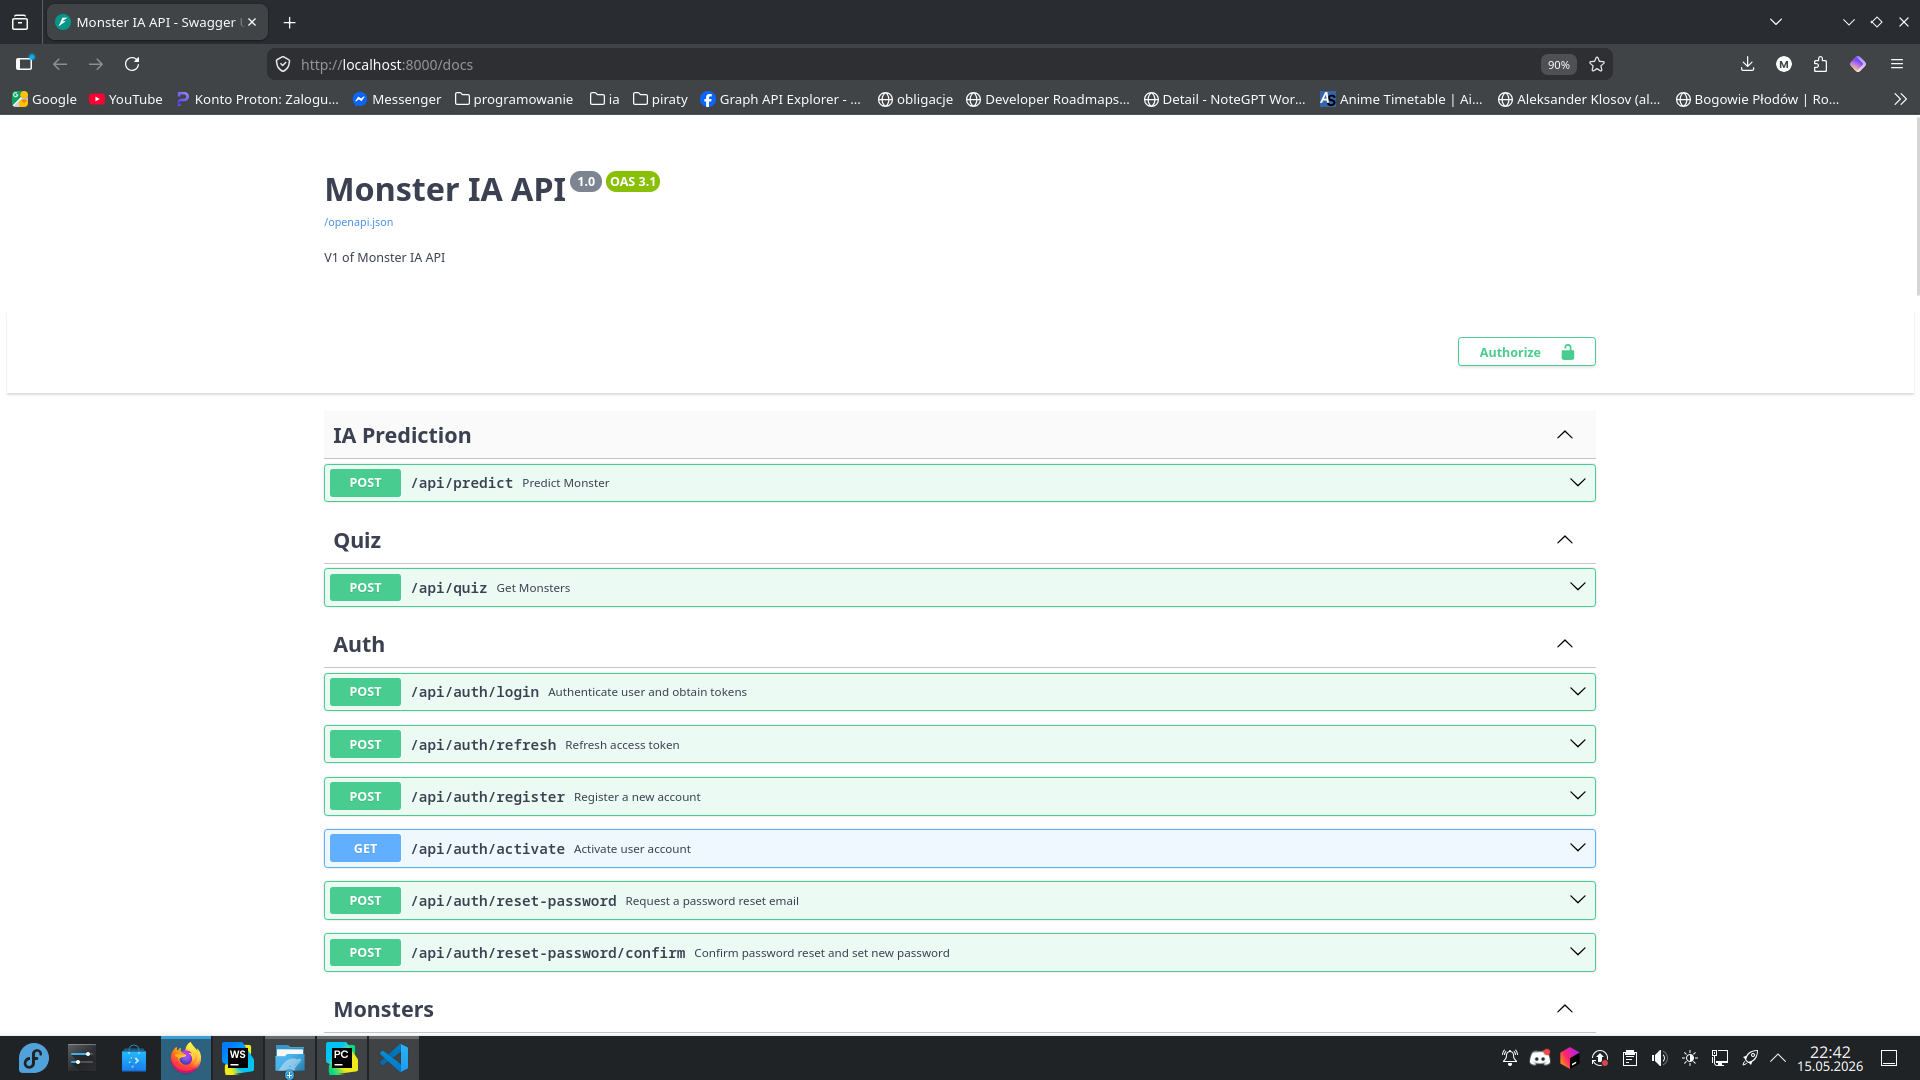
\includegraphics[width=1\textwidth]{swagger_1.png}
    \caption{Interaktywna dokumentacja REST API generowana przez framework FastAPI cz1.}
    \label{fig:backend}
\end{figure}

\begin{figure}[H]
    \centering
    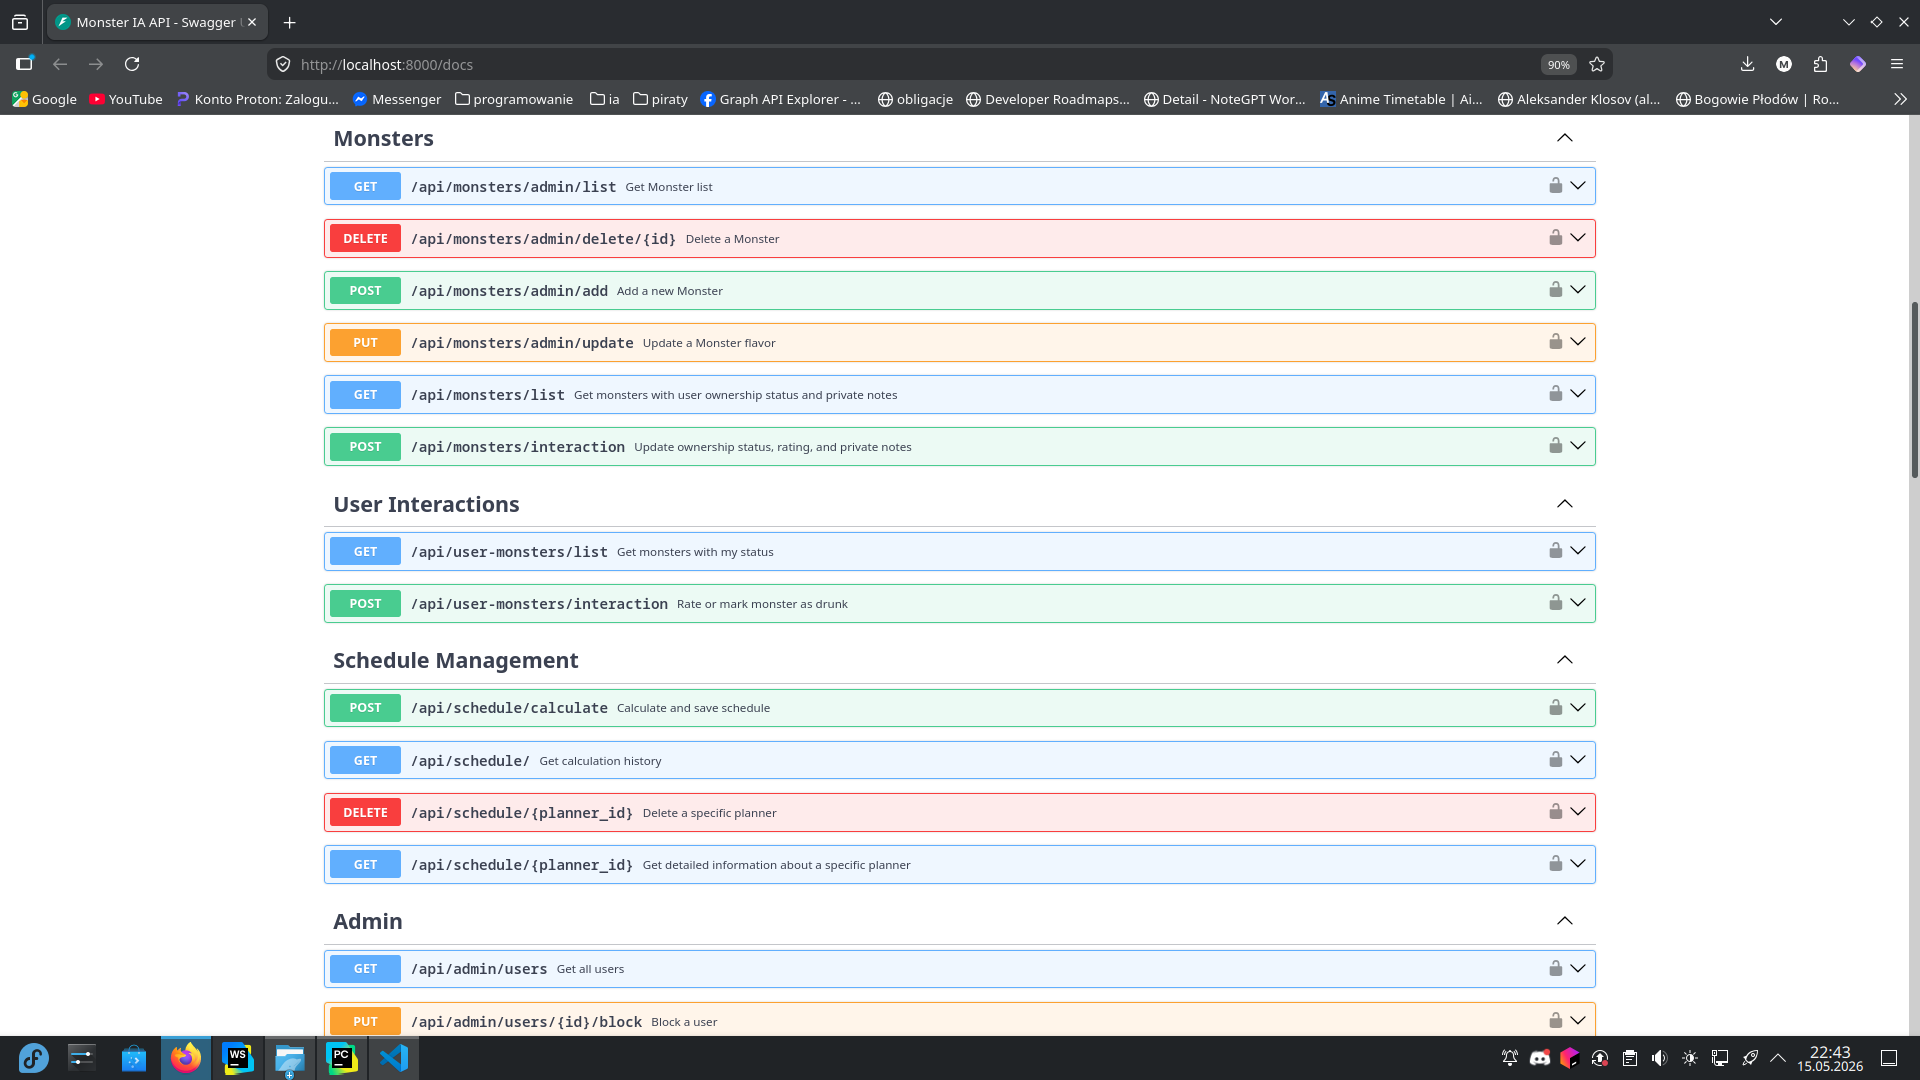
\includegraphics[width=1\textwidth]{swagger_2.png}
    \caption{Interaktywna dokumentacja REST API generowana przez framework FastAPI cz2.}
    \label{fig:backend}
\end{figure}

\begin{figure}[H]
    \centering
    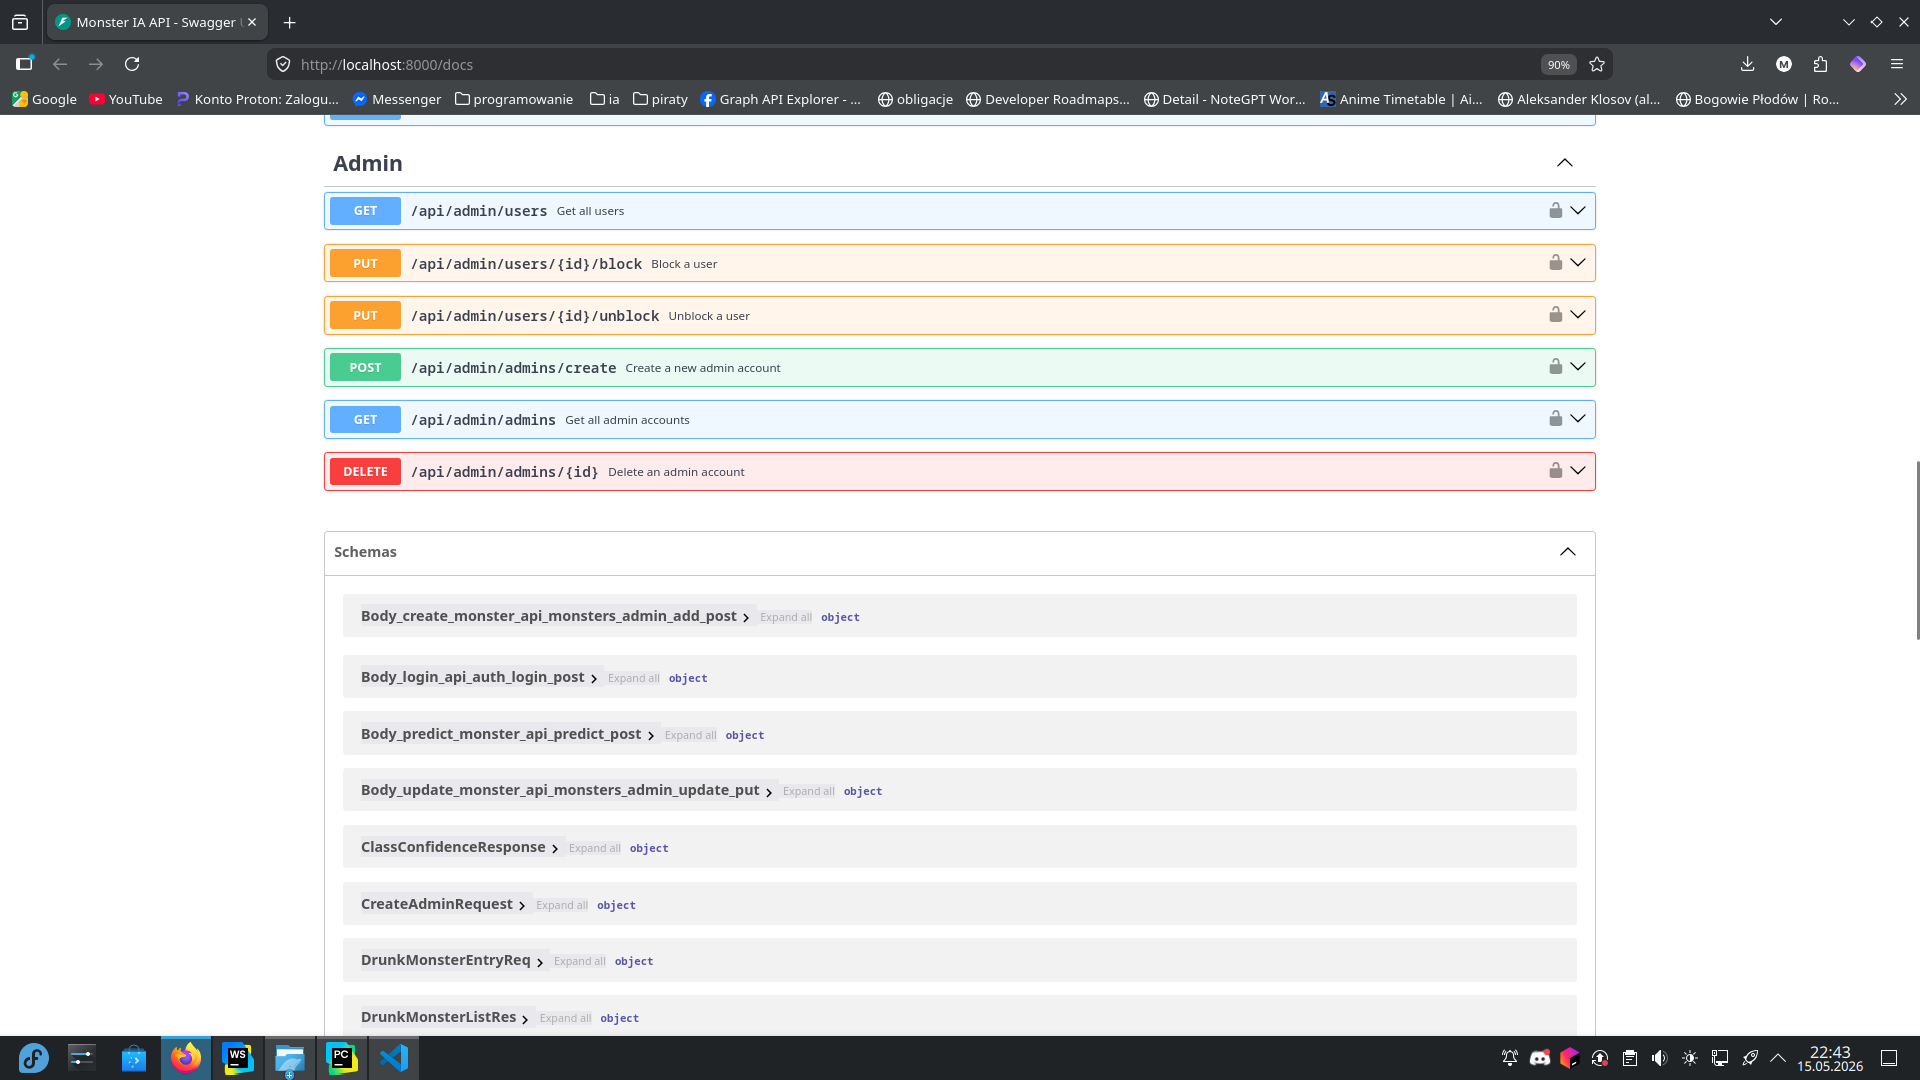
\includegraphics[width=1\textwidth]{swagger_3.png}
    \caption{Interaktywna dokumentacja REST API generowana przez framework FastAPI cz3.}
    \label{fig:backend}
\end{figure}

\section{Podsumowanie i wnioski ogólne}
Projekt MonsterAI z powodzeniem demonstruje praktyczne wykorzystanie trzech odmiennych metod sztucznej inteligencji: wizji komputerowej, algorytmów ewolucyjnych i systemów eksperckich, zamykając je w jednym, spójnym środowisku webowym. Technologia konteneryzacji Docker oraz asynchroniczność frameworka FastAPI sprawiły, że system jest nie tylko wydajny, ale i prosty we wdrożeniu. Zderzenie wymagań akademickich z komercyjnym podejściem do budowy oprogramowania (separacja frontend/backend, chmura S3) okazało się dużym sukcesem zespołu.

\newpage

\section{Wkład, udział i wnioski osobiste}
Poniżej znajduje się podsumowanie zaangażowania każdego z członków zespołu, weryfikujące zdobyte umiejętności oraz napotkane trudności.

\subsection{Mateusz Bogacz-Drewniak}
\textbf{Zakres prac:} 
\begin{itemize}
    \item Zarządzanie projektem
    \item Przygotowanie środowiska docker
    \item Implementacja bazy danych i zewnętrznych serwisów (MinIO, MailPit)
    \item Stworzenie systemu logowania, rejestracji, odzyskiwania hasła i endpointów CRUD
\end{itemize} 
\textbf{Plusy projektu:} 
\begin{itemize}
    \item Przekucie zdobytej wiedzy z zakresu zarządzania projektami w praktykę (m.in. poprzez stosowanie podobnych zasad w kołach naukowych).
    \item Zdobycie obszernej wiedzy na temat budowy sieci neuronowych i algorytmów genetycznych.
    \item Zapoznanie się z nowym frameworkiem webowym, zrozumienie jego filozofii oraz zdobycie podstawowych umiejętności tworzenia w nim aplikacji.
    \item Znaczne polepszenie zdolności zarządzania grupą.
\end{itemize}
\textbf{Minusy/Trudności:} 
\begin{itemize}
    \item Problemy z mechanizmami autoryzacji w FastAPI, co wymusiło zmianę logiki tworzenia systemu logowania opartego na JWT (framework ten zdaje się sprawdzać lepiej przy endpointach niewymagających autoryzacji).
    \item Niewspółmiernie duża ilość włożonej pracy oraz rzeczy do przygotowania w stosunku do przewidzianej nagrody za projekt (zaledwie 1 punkt ECTS).
    \item Trudności w zarządzaniu zespołem wynikające z faktu, że każdy z jego członków mierzy się z innymi problemami i sytuacjami życiowymi.
\end{itemize}

\subsection{Mateusz Chimkowski}
\textbf{Zakres prac:} \\
\textbf{Plusy projektu:} \\
\textbf{Minusy/Trudności:}

\subsection{Szymon Mikołajek}
\textbf{Zakres prac:} Frontend w React, budowa UI i UX, podłączenie API \\
\textbf{Plusy projektu:} \\
\textbf{Minusy/Trudności:}

\subsection{Paweł Kruk}
\textbf{Zakres prac:} Frontend w React, budowa UI i UX, podłączenie API \\
\textbf{Plusy projektu:} 
\begin{itemize}
    \item Sprawne wdrożenie Reacta w połączeniu z TypeScriptem, co znacząco usprawniło budowę interfejsu i ułatwiło zarządzanie stanem całej aplikacji.
    \item Zminimalizowanie ryzyka błędów podczas integracji z backendem dzięki zastosowaniu ścisłego typowania danych.
    \item Pomyślna integracja modułu sztucznej inteligencji do rozpoznawania obrazów (system sprawnie przetwarza zdjęcia i komunikuje się z API w czasie rzeczywistym).
    \item Oparcie aplikacji na modułowej architekturze kodu, co zapewnia wysoką skalowalność i pozwala na bezproblemowe dodawanie nowych funkcjonalności w przyszłości.
\end{itemize}
\textbf{Minusy/Trudności:} 
\begin{itemize}
    \item Problemy z synchronizacją pracy całego zespołu wynikające z różnych harmonogramów i dostępności czasowej poszczególnych osób.
    \item Słaba komunikacja na linii frontend-frontend, co skutkowało koniecznością wprowadzenia kilku mniejszych przeróbek interfejsu.
\end{itemize}

\subsection{Bartosz Dobroś}
\textbf{Zakres prac:}  \\
\textbf{Plusy projektu:} \\
\textbf{Minusy/Trudności:}

\newpage
\renewcommand{\lstlistlistingname}{Spis fragmentów kodu}

\listoffigures
\vspace{1cm}
\listoftables
\vspace{1cm}
\lstlistoflistings

\end{document}